\subsection{Background}
Legendrian knots are central objects in the study of 3-dimensional
contact manifolds. Classification of Legendrian knots is important in its
own right and also plays a prominent role in classifying 4-dimensional
Weinstein manifolds.

Classical Legendrian knot invariants are Thurston--Bennequin number and rotation
number~\cite{Gei2008} which distinguish the pair of Legendrian knots with the
same knot type. There are non-classical invariants including the Legendrian
contact algebra via the method of Floer theory~\cite{EGH2000, Che2002}, and
the space of constructible sheaves using microlocal
analysis~\cite{GKS2012,STZ2017}. These non-classical invariants distinguish
the Chekanov pair, a pair of Legendrian knots of type $m5_2$ having the same
classical invariants.


Recently, the study of exact Lagrangian fillings for Legendrian links has
been extremely plentiful. In the context of Legendrian contact algebra, an exact
Lagrangian filling gives an augmentation through the functorial view 
point~\cite{EHK2016}. There are several level of equivalence between 
augmentations
and the constructible sheaves for Legendrian links from counting to
categorical equivalence~\cite{NRSSZ2015}. 
Using these idea of
augmentations and constructible sheaves, people construct infinitely many fillings for certain Legendrian links~\cite{CG2020, GSW2020b,
CZ2020}. Here is the summarized list of methods of constructing Lagrangian
fillings for Legendrian links:
\begin{enumerate}
\item Decomposable Lagrangian fillings via pinching sequences and Legendrian loops \cite{EHK2016, Kal2006, CN2021}.
\item Alternating Legendrians and its conjugate Lagrangian fillings
\cite{STWZ2019}. 
\item Legendrian weaves via $N$-graphs and Legendrian mutations \cite{TZ2018, CZ2020}. 
\item Donaldson--Thomas transformation on augmentation varieties
\cite{SW2019, GSW2020a, GSW2020b}.
\end{enumerate}


Cluster algebras, introduced by Fomin and Zelevinsky~\cite{FZ1_2002}, play a crucial role in
the above constructions and applications. More precisely, the space of
augmentations and the moduli of constructible sheaves of microlocal rank one adapted to
Legendrian links admit structures of cluster pattern and $Y$-pattern, respectively~\cite{STWZ2019, SW2019, GSW2020a}. 
Note that a $Y$-seed of cluster algebra consists of a quiver whose vertices are
decorated with variables, called \emph{coefficients}. An involutory operation at each vertex,
called \emph{mutation}, generates all seeds of the $Y$-pattern.
The main point is to identify the
mutation in the $Y$-pattern and an operation in the space of Lagrangian
fillings. This geometric operation is deeply related to the Lagrangian surgery~\cite{Pol1991} and
the wall-crossing phenomenon~\cite{Aur2007}.


Indeed, a Legendrian torus link of type $(2,n)$ admits as many exact
Lagrangian fillings as Catalan number up to exact Lagrangian isotopy \cite{Pan2017, STWZ2019,
TZ2018}. Interestingly enough, the Catalan number is the number of seeds in a
cluster pattern of Dynkin type $\dynA_{n-1}$. 
There are also Legendrian links corresponding to finite Dynkin type $\dynD\dynE$, and affine Dynkin type $\exdynD\exdynE$ \cite{GSW2020b}.
A conjecture by Casals \cite[Conjecture~5.1]{Cas2020} says that the number of
distinct exact embedded Lagrangian fillings (up to exact Lagrangian isotopy) for
Legendrian links of type $\dynADE$ is exactly the same as the number of seeds
of the corresponding cluster algebras.

Furthermore, it is also conjectured by Casals \cite[Conjecture~5.4]{Cas2020} that for Legendrian links of type $\dynA_{2n-1}, \dynD_{n+1}, \dynE_6$ and $\dynD_4$, Lagrangian fillings having certain $\Z/2\Z$ or $\Z/3\Z$-symmetry form the cluster patterns of type $\dynB_n, \dynC_n, \dynF_4$ and $\dynG_2$, which are Dynkin diagrams obtained by \emph{folding} as explained in~\cite{FZ_Ysystem03}.


\subsection{The results}
\subsubsection{Lagrangian fillings for Legendrians of type $\dynADE$ or $\exdynD\exdynE$}
Our main result is that there are at least as many Lagrangian fillings for
Legendrian links of finite type as seeds in the corresponding cluster structures. We deal with $N$-graphs introduced by Casals and Zaslow \cite{CZ2020} to
construct the Lagrangian fillings. An $N$-graph $\ngraph$ on $\disk^2$ gives
a Legendrian surface $\Legendrian(\ngraph)$ in $J^1\disk^2$ while the
boundary $\boundary \ngraph$ on $\sphere^1$ induces a Legendrian link~$\legendrian(\boundary \ngraph)$. Then projection of $\Legendrian(\ngraph)$
along the Reeb direction becomes a Lagrangian filling of~$\legendrian(\boundary \ngraph)$.

As mentioned above, we interpret an $N$-graph as a $Y$-seed in the corresponding
$Y$-pattern. A one-cycle in the Legendrian surface
$\Legendrian(\ngraph)$ corresponds to a vertex of the quiver, and a signed
intersection between one-cycles gives an arrow between corresponding
vertices. From constructible sheaves adapted to $\Legendrian(\ngraph)$, one
can assign a monodromy to each one-cycle which becomes the coefficient at each vertex.

There is an operation so called a \emph{Legendrian mutation}
$\mutation_\cycle$ on an $N$-graph $\ngraph$ along one-cycle $[\cycle]\in
H_1(\Legendrian(\ngraph))$ which is the counterpart of the mutation on the
$Y$-pattern, see Proposition~\ref{proposition:equivariance of mutations}. The
delicate and challenging part is that we do not know whether Legendrian
mutations are always possible or not. Simply put, this is because the
mutation in cluster side is algebraic, whereas the Legendrian mutation is
rather geometric.

The main idea of our construction is to consider $N$-graphs $\ngraph(a,b,c)$ and $\ngraph(\exdynD_n)$ bounding Legendrian links $\legendrian(a,b,c)$ and $\legendrian(\exdynD_n)$, respectively.

\begin{align*}
\legendrian(a,b,c)=
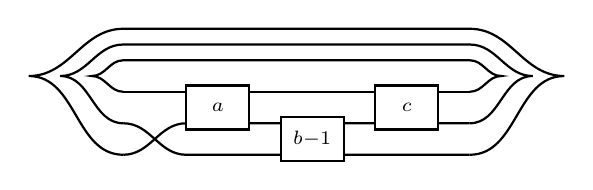
\begin{tikzpicture}[baseline=5ex,scale=0.8]
\draw[thick] (0,0) to[out=0,in=180] (1,0.5) (2,0.5) to (2.5,0.5) (3.5,0.5) to (4,0.5) (5,0.5) to (5.5,0.5);
\draw[thick] (0,0.5) to[out=0,in=180] (1,0) to (2.5,0) (3.5,0) to (5.5,0);
\draw[thick] (0,1) to[out=0,in=180] (1,1) (2,1) to (4,1) (5,1) to (5.5,1);
\draw[thick] (1,0.4) rectangle node {$\scriptstyle a$} (2, 1.1);
\draw[thick] (2.5,-0.1) rectangle node {$\scriptstyle{b-1}$} (3.5, 0.6);
\draw[thick] (4,0.4) rectangle node {$\scriptstyle c$} (5, 1.1);
\draw[thick] (0,1) to[out=180, in=0] (-0.5,1.25) to[out=0,in=180] (0,1.5) to (5.5,1.5) to[out=0,in=180] (6,1.25) to[out=180,in=0] (5.5,1);
\draw[thick] (0,0.5) to[out=180, in=0] (-1,1.25) to[out=0,in=180] (0,1.75) to (5.5,1.75) to[out=0,in=180] (6.5,1.25) to[out=180,in=0] (5.5,0.5);
\draw[thick] (0,0) to[out=180, in=0] (-1.5,1.25) to[out=0,in=180] (0,2) to (5.5,2) to[out=0,in=180] (7,1.25) to[out=180,in=0] (5.5,0);
\end{tikzpicture}
\end{align*}

\begin{align*}
\legendrian({{\exdynD}_n})=
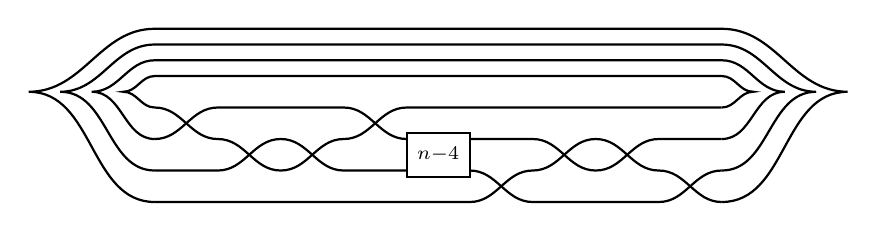
\begin{tikzpicture}[baseline=-0.5ex,scale=0.8]
%braidpart
\draw[thick] (0,0) to[out=0,in=180] (1,-0.5) to[out=0,in=180] (2,-1) to[out=0,in=180] (3,-0.5) to[out=0,in=180] (4,0) to[out=0,in=180] (9,0);
\draw[thick] (0,-0.5) to[out=0,in=180] (1,0) to[out=0,in=180] (3,0) to[out=0,in=180] (4,-0.5) (5,-0.5) to[out=0,in=180] (6,-0.5) to[out=0,in=180] (7,-1) to[out=0,in=180] (8,-0.5) to[out=0,in=180] (9,-0.5);
\draw[thick] (0,-1) to[out=0,in=180] (1,-1) to[out=0,in=180] (2,-0.5) to[out=0,in=180] (3,-1) to[out=0,in=180] (4,-1) (5,-1) to[out=0,in=180] (6,-1.5) to[out=0,in=180] (8,-1.5) to[out=0,in=180] (9,-1);
\draw[thick] (0,-1.5) to[out=0,in=180] (5,-1.5) to[out=0,in=180] (6,-1) to[out=0,in=180] (7,-0.5) to[out=0,in=180] (8,-1) to[out=0,in=180] (9,-1.5);
\draw[thick] (4,-0.4) rectangle node {$\scriptstyle{n-4}$} (5, -1.1);
%closure part
\draw[thick] (0,0) to[out=180,in=0] (-0.5,0.25) to[out=0,in=180] (0,0.5) to[out=0,in=180] (9,0.5) to[out=0,in=180] (9.5,0.25) to[out=180,in=0] (9,0);
\draw[thick] (0,-0.5) to[out=180,in=0] (-1,0.25) to[out=0,in=180] (0,0.75) to[out=0,in=180] (9,0.75) to[out=0,in=180] (10,0.25) to[out=180,in=0] (9,-0.5);
\draw[thick] (0,-1) to[out=180,in=0] (-1.5,0.25) to[out=0,in=180] (0,1) to[out=0,in=180] (9,1) to[out=0,in=180] (10.5,0.25) to[out=180,in=0] (9,-1);
\draw[thick] (0,-1.5) to[out=180,in=0] (-2,0.25) to[out=0,in=180] (0,1.25) to[out=0,in=180] (9,1.25) to[out=0,in=180] (11,0.25) to[out=180,in=0] (9,-1.5);
\end{tikzpicture}
\end{align*}
Note that the above Legendrians $\legendrian(a,b,c)$ and $\legendrian(\exdynD_n)$ can be obtained by ($-1$)-closure of the following braids, respectively,
\begin{align*}
\beta(a,b,c)&=\sigma_2\sigma_1^{a+1}\sigma_2\sigma_1^{b+1}\sigma_2\sigma_1^{c+1},&
\beta(\exdynD_n)&=\left(\sigma_2\sigma_1^3\sigma_2\sigma_1^3\sigma_2\sigma_1^k\sigma_3\right)\cdot\left(\sigma_2\sigma_1^3\sigma_2\sigma_1^3\sigma_2\sigma_1^\ell\sigma_3\right),
\end{align*}
where $k=\lfloor \frac{n-3}2\rfloor$ and $\ell=\lfloor \frac{n-4}2\rfloor$, see Section~\ref{sec:N-graph of finite or affine type}.
Those braids provide boundary data of the following $N$-graphs which represent exact Lagrangian fillings of corresponding Legendrian links:

\begin{figure}[ht]
\subfigure[$(\ngraph(a,b,c),\nbasis(a,b,c))$\label{N-graph(a,b,c)}]{
$
\begin{tikzpicture}[baseline=-.5ex,scale=0.6]
\draw[thick] (0,0) circle (3cm);
%\draw[line cap=round, line width=5, opacity=0.5] (3,0) -- (-1,0) (60:1) -- (100:3);
\draw[color=cyclecolor2, line cap=round, line width=5, opacity=0.5] (60:1) -- (50:1.5) (70:1.75) -- (50:2) (180:1) -- (170:1.5) (190:1.75) -- (170:2) (300:1) -- (290:1.5) (310:1.75) -- (290:2);
\draw[color=cyclecolor1, line cap=round, line width=5, opacity=0.5] (0,0) -- (60:1) (0,0) -- (180:1) (0,0) -- (300:1) (50:1.5) -- (70:1.75) (170:1.5) -- (190:1.75) (290:1.5) -- (310:1.75);
\draw[red, thick] (0,0) -- (0:3) (0,0) -- (120:3) (0,0) -- (240:3);
\draw[blue, thick, fill] (0,0) -- (60:1) circle (2pt) -- (100:3) (60:1) -- (50:1.5) circle (2pt) -- (20:3) (50:1.5) -- (70:1.75) circle (2pt) -- (80:3) (70:1.75) -- (50:2) circle (2pt) -- (40:3);
\draw[blue, thick, dashed] (50:2) -- (60:3);
\draw[blue, thick, fill] (0,0) -- (180:1) circle (2pt) -- (220:3) (180:1) -- (170:1.5) circle (2pt) -- (140:3) (170:1.5) -- (190:1.75) circle (2pt) -- (200:3) (190:1.75) -- (170:2) circle (2pt) -- (160:3);
\draw[blue, thick, dashed] (170:2) -- (180:3);
\draw[blue, thick, fill] (0,0) -- (300:1) circle (2pt) -- (340:3) (300:1) -- (290:1.5) circle (2pt) -- (260:3) (290:1.5) -- (310:1.75) circle (2pt) -- (320:3) (310:1.75) -- (290:2) circle (2pt) -- (280:3);
\draw[blue, thick, dashed] (290:2) -- (300:3);
\draw[thick, fill=white] (0,0) circle (2pt);
\curlybrace[]{10}{110}{3.2};
\draw (300:3.5) node[rotate=30] {\small ${c+1}$};
\curlybrace[]{130}{230}{3.2};
\draw (180:3.5) node[rotate=90] {\small $b+1$};
\curlybrace[]{250}{350}{3.2};
\draw (60:3.5) node[rotate=-30] {\small $a+1$};
\end{tikzpicture}
$}
\qquad
\subfigure[$(\ngraph(\exdynD_{n}),\nbasis(\exdynD_{n}))$\label{N-graph(Dn)}]{
$
\begin{tikzpicture}[baseline=-.5ex,scale=0.6]
\draw[rounded corners=5, thick] (-6.5, -2.5) rectangle (6.5, 2.5);
\draw (0.5, -2.5) node[above] {$\cdots$} 
(-0.5, -2.5) node[below] {$\underbrace{\hphantom{\hspace{3cm}}}_{k}$};
\draw (1.5, 2.5) node[below] {$\cdots$} 
(0.5, 2.5) node[above] {$\overbrace{\hphantom{\hspace{3cm}}}^{\ell}$};
\clip[rounded corners=5] (-6.5, -2.5) rectangle (6.5, 2.5);
\draw[cyclecolor1, opacity=0.5, line cap=round, line width=5] 
(-3.5, 0) -- (-2.5, 0) (-3.5, 0) -- (-4.5, 1) (-3.5, 0) -- (-4.5, -1)
(-1.5, 0) -- (-0.5, 0)
(0.5, 0) -- (1.5, 0)
(3.5, 0) -- (2.5, 0) (3.5, 0) -- (4.5, 1) (3.5, 0) -- (4.5, -1)
;
\draw[cyclecolor2, opacity=0.5, line cap=round, line width=5] 
(-4.5, 1) -- (-5.5, 1)
(-4.5, -1) -- (-4.5, -1.75)
(-1.5, 0) -- (-2.5, 0)
(-0.5, 0) -- (0.5, 0)
(1.5, 0) -- (2.5, 0)
(4.5, 1) -- (4.5, 1.75)
(4.5, -1) -- (5.5, -1)
;
\foreach \i in {0, 180} {
\begin{scope}[rotate=\i]
\draw[thick, green] (-2.5, 2.5) -- (0,0);
\draw[thick, red] 
(-3.5, -2.5) -- (-3.5, 2.5)
(-6.5, 0) -- (-3.5, 0)
;
\draw[thick, blue, fill]
(-2.5, -2.5) -- (-2.5,0) circle (2pt)
(-0.5, -2.5) -- (-0.5,0) circle (2pt)
(1.5, -2.5) -- (1.5,0) circle (2pt)
;
\draw[thick, blue, fill] 
%
(-3.5, 0) -- (3.5, 0)
(-3.5, 0) -- (-4.5, 1) circle (2pt) -- (-4.5, 2.5)
(-4.5, 1) -- (-6.5, 1)
(-5.5, 1) circle (2pt) -- (-5.5, 2.5)
%
(-3.5, 0) -- (-4.5, -1) circle (2pt) -- (-4.5, -2.5)
(-4.5, -1) -- (-6.5, -1)
(-4.5, -1.73) circle (2pt) -- (-6.5, -1.73)
;
\end{scope}
}
\draw[thick, fill=white] (-3.5, 0) circle (2pt) (3.5, 0) circle (2pt);
\end{tikzpicture}
$}
\caption{Pairs of $N$-graphs and tuples of cycles}
\label{fig:N-graphs of (a,b,c) and Dn}
\end{figure}

\noindent Here, the \colorbox{cyclecolor1!50!}{\cyclecolornamefirst}- and \colorbox{cyclecolor2!50!}{\cyclecolornamesecond}-shaded edges indicate a tuple of one-cycles $\nbasis$ in the corresponding Legendrian surface.
See~\S\ref{sec:1-cycles in Legendrian weaves} for the detail.



The Legendrians $\legendrian(a,b,c), \legendrian(\exdynD_n)$ are the rainbow closure of \emph{positive braids}. 
By the work of Shen--Weng \cite{SW2019}, it is direct to check that 
the corresponding cluster structure of Legendrian $\legendrian(\dynX)$ is 
indeed of type $\dynX$ for $\dynX\in\{\dynA,\dynD,\dynE,\exdynD,\exdynE\}$. More precisely, the coordinate 
ring of the moduli space $\cM_1(\legendrian(\dynX))$ of microlocal rank one 
sheaves in $\Sh^\bullet_{\legendrian(\dynX)}(\R^2)$ admits the aforementioned 
$Y$-pattern structure.
By the way, the (candidate) Legendrians of type $\exdynA$ are not the rainbow 
closure of positive braids, in general. 
Indeed, Casals--Ng~\cite{CN2021} considered a Legendrian link of type 
$\exdynA_{1,1}$ which is not the rainbow closure of a  positive braid. 
So we can not directly apply the subsequent argument to Legendrians of type 
$\exdynA$.

To prove the realizability of each $Y$-seed in the corresponding $Y$-pattern, we use an induction argument on the rank of the type $\dynX$. 
More precisely, for each $Y$-pattern, we consider the \emph{exchange graph}, whose vertices are the $Y$-seeds and whose edges connect the vertices related by a single mutation. 
It has been known that the exchange graph of a $Y$-pattern is determined by the Dynkin type $\dynX$ of the $Y$-pattern when $\dynX$ is finite or affine (cf. Propositions~\ref{thm_exchange_graph_Dynkin} and~\ref{prop_Y-pattern_exchange_graph}). Because of this, we denote by $\exchange(\Roots(\dynX))$ the exchange graph of a $Y$-pattern of type $\dynX$.
Here, $\Roots(\dynX)$ is the root system of type $\dynX$. Note that when $\dynX$ is of finite type, the exchange graph $\exchange(\Roots(\dynX))$ becomes the one-skeleton of a polytope, called the (\emph{generalized}) \emph{associahedron} (see Figures~\ref{fig_asso_A3_intro} and~\ref{fig_asso_D4}).
\begin{figure}[ht]
% \todo{Draw A3 associahedron}
\tdplotsetmaincoords{110}{-30}
\begin{tikzpicture}%
[tdplot_main_coords,
% 	x={(0.497546cm, 0.859773cm)},
% y={(-0.106336cm, -0.071189cm)},
% z={(0.860895cm, -0.505690cm)},
%scale= 2,
% [x={(-0.495892cm, -0.532283cm)},
% y={(0.868384cm, -0.303848cm)},
% z={(-0.000125cm, 0.790159cm)},
scale=0.700000,
back/.style={loosely dotted, thin},
edge/.style={color=black, thick},
facet/.style={fill=blue!95!black,fill opacity=0.100000},
vertex/.style={inner sep=1pt,circle,fill=black,thick,anchor=base},
gvertex/.style={inner sep=1.2pt,circle,draw=green!25!black,fill=green!75!black,thick,anchor=base}]
%% Coordinate of the vertices:
%%
\coordinate (1) at (-0.50000, -1.50000, 2.00000);
\coordinate (2) at (1.50000, 1.50000, -2.00000);
\coordinate (3) at (0.50000, 0.50000, 1.00000);
\coordinate (4) at (0.50000, 1.50000, 0.00000);
\coordinate (5) at (1.50000, 1.50000, -1.00000);
\coordinate (6) at (-0.50000, -0.50000, 2.00000);
\coordinate (7) at (1.50000, 0.50000, 0.00000);
\coordinate (8) at (1.50000, -1.50000, 0.00000);
\coordinate (9) at (1.50000, -1.50000, -2.00000);
\coordinate (10) at (-1.50000, -1.50000, -2.00000);
\coordinate (11) at (-1.50000, -1.50000, 2.00000);
\coordinate (12) at (-1.50000, 1.50000, -2.00000);
\coordinate (13) at (-1.50000, 1.50000, 0.00000);
\coordinate (14) at (-1.50000, -0.50000, 2.00000);

%% fill some facets
\fill[cyclecolor1, opacity = 0.3] (10)--(12)--(13)--(14)--(11)--cycle;
\fill[cyclecolor2, opacity = 0.2] (10)--(9)--(8)--(1)--(11)--cycle;
\fill[yellow, opacity = 0.3] (10)--(9)--(2)--(12)--cycle;

%%
%%
%% Drawing edges in the back
%%
\draw[edge,back] (9) -- (10);
\draw[edge,back] (10) -- (11);
\draw[edge,back] (10) -- (12);
%%
%%
%% Drawing vertices in the back
%%
\node[vertex] at (10)     {};

% %%
%%
%% Drawing edges in the front
%%
\draw[edge] (1) -- (6);
\draw[edge] (1) -- (8);
\draw[edge] (1) -- (11);
\draw[edge] (2) -- (5);
\draw[edge] (2) -- (9);
\draw[edge] (2) -- (12);
\draw[edge] (3) -- (4);
\draw[edge] (3) -- (6);
\draw[edge] (3) -- (7);
\draw[edge] (4) -- (5);
\draw[edge] (4) -- (13);
\draw[edge] (5) -- (7);
\draw[edge] (6) -- (14);
\draw[edge] (7) -- (8);
\draw[edge] (8) -- (9);
\draw[edge] (11) -- (14);
\draw[edge] (12) -- (13);
\draw[edge] (13) -- (14);
%%
%%
%% Drawing the vertices in the front
%%
\node[vertex] at (1)     {};
\node[vertex] at (2)     {};
\node[vertex] at (3)     {};
\node[vertex] at (4)     {};
\node[vertex] at (5)     {};
\node[vertex] at (6)     {};
\node[vertex] at (7)     {};
\node[vertex] at (8)     {};
\node[vertex] at (9)     {};
\node[vertex] at (11)     {};
\node[vertex] at (12)     {};
\node[vertex] at (13)     {};
\node[vertex] at (14)     {};

\foreach \g in {10, 6, 5} {
\node[gvertex] at (\g) {};
}
%%
%%
%
%\foreach \x in {1,...,14}{
%\node at (\x) {\x};
%}

\end{tikzpicture}%
\hspace{1cm}%
%%
\begin{tikzpicture}%
[tdplot_main_coords,
% 	x={(0.497546cm, 0.859773cm)},
% y={(-0.106336cm, -0.071189cm)},
% z={(0.860895cm, -0.505690cm)},
%scale= 2,
% [x={(-0.495892cm, -0.532283cm)},
% y={(0.868384cm, -0.303848cm)},
% z={(-0.000125cm, 0.790159cm)},
scale=0.700000,
back/.style={loosely dotted, thin},
edge/.style={color=black, thick},
facet/.style={fill=blue!95!black,fill opacity=0.100000},
vertex/.style={inner sep=1pt,circle,fill=black,thick,anchor=base},
gvertex/.style={inner sep=1.2pt,circle,draw=green!25!black,fill=green!75!black,thick,anchor=base}]
%% Coordinate of the vertices:
%%
\coordinate (1) at (-0.50000, -1.50000, 2.00000);
\coordinate (2) at (1.50000, 1.50000, -2.00000);
\coordinate (3) at (0.50000, 0.50000, 1.00000);
\coordinate (4) at (0.50000, 1.50000, 0.00000);
\coordinate (5) at (1.50000, 1.50000, -1.00000);
\coordinate (6) at (-0.50000, -0.50000, 2.00000);
\coordinate (7) at (1.50000, 0.50000, 0.00000);
\coordinate (8) at (1.50000, -1.50000, 0.00000);
\coordinate (9) at (1.50000, -1.50000, -2.00000);
\coordinate (10) at (-1.50000, -1.50000, -2.00000);
\coordinate (11) at (-1.50000, -1.50000, 2.00000);
\coordinate (12) at (-1.50000, 1.50000, -2.00000);
\coordinate (13) at (-1.50000, 1.50000, 0.00000);
\coordinate (14) at (-1.50000, -0.50000, 2.00000);

%% fill some facets
\fill[cyclecolor1, opacity = 0.3] (6)--(3)--(7)--(8)--(1)--cycle;
\fill[cyclecolor2, opacity = 0.2] (6)--(3)--(4)--(13)--(14)--cycle;
\fill[yellow, opacity = 0.3] (6)--(1)--(11)--(14)--cycle;

%%
%%
%% Drawing edges in the back
%%
\draw[edge,back] (9) -- (10);
\draw[edge,back] (10) -- (11);
\draw[edge,back] (10) -- (12);
%%
%%
%% Drawing vertices in the back
%%
\node[vertex] at (10)     {};

% %%
%%
%% Drawing edges in the front
%%
\draw[edge] (1) -- (6);
\draw[edge] (1) -- (8);
\draw[edge] (1) -- (11);
\draw[edge] (2) -- (5);
\draw[edge] (2) -- (9);
\draw[edge] (2) -- (12);
\draw[edge] (3) -- (4);
\draw[edge] (3) -- (6);
\draw[edge] (3) -- (7);
\draw[edge] (4) -- (5);
\draw[edge] (4) -- (13);
\draw[edge] (5) -- (7);
\draw[edge] (6) -- (14);
\draw[edge] (7) -- (8);
\draw[edge] (8) -- (9);
\draw[edge] (11) -- (14);
\draw[edge] (12) -- (13);
\draw[edge] (13) -- (14);
%%
%%
%% Drawing the vertices in the front
%%
\node[vertex] at (1)     {};
\node[vertex] at (2)     {};
\node[vertex] at (3)     {};
\node[vertex] at (4)     {};
\node[vertex] at (5)     {};
\node[vertex] at (6)     {};
\node[vertex] at (7)     {};
\node[vertex] at (8)     {};
\node[vertex] at (9)     {};
\node[vertex] at (11)     {};
\node[vertex] at (12)     {};
\node[vertex] at (13)     {};
\node[vertex] at (14)     {};

\foreach \g in {10, 6, 5} {
\node[gvertex] at (\g) {};
}
%%
%%

%\foreach \x in {1,...,14}{
%\node at (\x) {\x};
%}

\end{tikzpicture} %
\hspace{1cm}%
\begin{tikzpicture}%
[tdplot_main_coords,
% 	x={(0.497546cm, 0.859773cm)},
% y={(-0.106336cm, -0.071189cm)},
% z={(0.860895cm, -0.505690cm)},
%scale= 2,
% [x={(-0.495892cm, -0.532283cm)},
% y={(0.868384cm, -0.303848cm)},
% z={(-0.000125cm, 0.790159cm)},
scale=0.700000,
back/.style={loosely dotted, thin},
edge/.style={color=black, thick},
facet/.style={fill=blue!95!black,fill opacity=0.100000},
vertex/.style={inner sep=1pt,circle,fill=black,thick,anchor=base},
gvertex/.style={inner sep=1.2pt,circle,draw=green!25!black,fill=green!75!black,thick,anchor=base}]
%% Coordinate of the vertices:
%%
\coordinate (1) at (-0.50000, -1.50000, 2.00000);
\coordinate (2) at (1.50000, 1.50000, -2.00000);
\coordinate (3) at (0.50000, 0.50000, 1.00000);
\coordinate (4) at (0.50000, 1.50000, 0.00000);
\coordinate (5) at (1.50000, 1.50000, -1.00000);
\coordinate (6) at (-0.50000, -0.50000, 2.00000);
\coordinate (7) at (1.50000, 0.50000, 0.00000);
\coordinate (8) at (1.50000, -1.50000, 0.00000);
\coordinate (9) at (1.50000, -1.50000, -2.00000);
\coordinate (10) at (-1.50000, -1.50000, -2.00000);
\coordinate (11) at (-1.50000, -1.50000, 2.00000);
\coordinate (12) at (-1.50000, 1.50000, -2.00000);
\coordinate (13) at (-1.50000, 1.50000, 0.00000);
\coordinate (14) at (-1.50000, -0.50000, 2.00000);

%% fill some facets
\fill[cyclecolor1, opacity = 0.3] (4)--(5)--(2)--(12)--(13)--cycle;
\fill[cyclecolor2, opacity = 0.2] (5)--(2)--(9)--(8)--(7)--cycle;
\fill[yellow, opacity = 0.3] (3)--(4)--(5)--(7)--cycle;

%%
%%
%% Drawing edges in the back
%%
\draw[edge,back] (9) -- (10);
\draw[edge,back] (10) -- (11);
\draw[edge,back] (10) -- (12);
%%
%%
%% Drawing vertices in the back
%%
\node[vertex] at (10)     {};

% %%
%%
%% Drawing edges in the front
%%
\draw[edge] (1) -- (6);
\draw[edge] (1) -- (8);
\draw[edge] (1) -- (11);
\draw[edge] (2) -- (5);
\draw[edge] (2) -- (9);
\draw[edge] (2) -- (12);
\draw[edge] (3) -- (4);
\draw[edge] (3) -- (6);
\draw[edge] (3) -- (7);
\draw[edge] (4) -- (5);
\draw[edge] (4) -- (13);
\draw[edge] (5) -- (7);
\draw[edge] (6) -- (14);
\draw[edge] (7) -- (8);
\draw[edge] (8) -- (9);
\draw[edge] (11) -- (14);
\draw[edge] (12) -- (13);
\draw[edge] (13) -- (14);
%%
%%
%% Drawing the vertices in the front
%%
\node[vertex] at (1)     {};
\node[vertex] at (2)     {};
\node[vertex] at (3)     {};
\node[vertex] at (4)     {};
\node[vertex] at (5)     {};
\node[vertex] at (6)     {};
\node[vertex] at (7)     {};
\node[vertex] at (8)     {};
\node[vertex] at (9)     {};
\node[vertex] at (11)     {};
\node[vertex] at (12)     {};
\node[vertex] at (13)     {};
\node[vertex] at (14)     {};

\foreach \g in {10, 6, 5} {
\node[gvertex] at (\g) {};
}
%%
%%
%
%\foreach \x in {1,...,14}{
%\node at (\x) {\x};
%}

\end{tikzpicture}
\caption{The type $\dynA_3$ associahedron}\label{fig_asso_A3_intro}
\end{figure}

A (fixed) sequence of mutations corresponding to a chosen Coxeter element provides an action on the exchange graph. We call this specific sequence of mutations a \emph{Coxeter mutation} $\mutation_{\quiver}$. The orbit of the initial seed is called \emph{bipartite belt}. The green dots in Figure~\ref{fig_asso_A3_intro} present the elements of the bipartite belt.
We notice that the facets meeting at the initial seed correspond to the exchange graphs $\exchange(\Roots(\dynX\setminus \{i\}))$. In Figure~\ref{fig_asso_A3_intro}, there are two pentagons and one square intersecting a green dot. Indeed, a pentagon is the type $\dynA_2$ generalized associahedron; a square is the type $\dynA_1 \times \dynA_1$ generalized associahedron. Moreover, by applying the Coxeter mutation on these facets iteratively, one can obtain all facets in the associahedron. 
Even though we do not have a polytope model for the exchange graph of affine type, similar properties hold, that is, one can reach any $Y$-seed in the exchange graph from the initial seed by taking Coxeter mutations and then applying a certain sequence of mutations omitting at least one vertex. 

The following good properties of the above pairs $(\ngraph(a,b,c),\nbasis(a,b,c))$ and $(\ngraph(\exdynD_{n}),\nbasis(\exdynD_{n}))$ play a crucial role in interpreting the Coxeter mutation $\qcoxeter$ in terms of $N$-graphs:
\begin{enumerate}
\item The geometric and algebraic intersection numbers between chosen one-cycles coincide. 
\item The corresponding quivers $\quiver(a,b,c)$, $\quiver(\exdynD_n)$ are bipartite, see~\S\ref{sec:N-graphs and seeds} for the details. 
\end{enumerate}
The property (2) naturally splits $\nbasis$ into two subsets $\nbasis_+$ and $\nbasis_-$.
In Figure~\ref{fig:N-graphs of (a,b,c) and Dn}, they consist of \colorbox{cyclecolor1!50!}{\cyclecolornamefirst}- and \colorbox{cyclecolor2!50!}{\cyclecolornamesecond}-shaded edges, respectively. 
Then the property (1) enables us to perform the \emph{Legendrian Coxeter mutation}, which is the $N$-graph realization of the Coxeter mutation defiend by the sequence of Legendrian mutations:
\[
\ncoxeter=\prod_{\cycle \in \nbasis_+} \mutation_{\cycle}\cdot\prod_{\cycle\in \nbasis_-} \mutation_{\cycle}.
\]
Then the resulting $N$-graphs $\ncoxeter(\ngraph(a,b,c),\nbasis(a,b,c))$ and $\ncoxeter(\ngraph(\exdynD_n),\nbasis(\exdynD_n))$ become the
$N$-graphs shown in Figure~\ref{figure:intro_Legendrian Coxeter mutation} up to a sequence of Move~\Move{II} in Figure~\ref{fig:move1-6}.
\begin{figure}[ht]
\subfigure[$\ncoxeter(\ngraph(a,b,c),\nbasis(a,b,c))$\label{ncoxeter_n(a,b,c)}]{
$
\begin{tikzpicture}[baseline=-.5ex,xscale=0.5, yscale=0.5]
\draw[thick] (0,0) circle (5cm);
\draw[dashed]  (0,0) circle (3cm);
\fill[opacity=0.1, even odd rule] (0,0) circle (3) (0,0) circle (5);
\foreach \i in {1,2,3} {
\begin{scope}[rotate=\i*120]
\draw[color=cyclecolor2, line cap=round, line width=5, opacity=0.5] (60:1) -- (50:1.5) (70:1.75) -- (50:2);
\draw[color=cyclecolor1, line cap=round, line width=5, opacity=0.5] (0,0) -- (60:1) (50:1.5) -- (70:1.75);
%
\draw[blue, thick, rounded corners] (0,0) -- (0:3.4) to[out=-75,in=80] (-40:4);
\draw[red, thick, fill] (0,0) -- (60:1) circle (2pt) (60:1) -- (50:1.5) circle (2pt) -- (70:1.75) circle (2pt) -- (50:2) circle (2pt);
\draw[red, thick, dashed, rounded corners] (50:2) -- (60:2.8) -- (60:3.3) to[out=0,in=220] (40:4);
\draw[red, thick, rounded corners] (50:2) -- (40:2.8) -- (40:3.3) to[out=-20,in=200] (20:4) (70:1.75) -- (80:2.8) -- (80:3.3) to[out=20,in=240] (60:4) (60:1) -- (100:2.8) -- (100:3.3) to[out=40,in=260] (80:4);
\draw[red, thick, rounded corners] (50:1.5) -- (20:3) -- (20:3.5) to[out=-70,in=50] (-40:4) (20:4) to[out=-50,in=120] (0:4.5) -- (0:5);
\draw[red, thick] (20:4) to[out=100,in=-40] (40:4) (60:4) to[out=140,in=0] (80:4);
\draw[blue, thick] (20:5) -- (20:4) to[out=140,in=-80] (40:4) (60:5) -- (60:4) to[out=180,in=-40] (80:4) -- (80:5);
\draw[thick, dotted] (40:4) arc (40:60:4);
\draw[blue, thick, rounded corners] (20:4) to[out=-70,in=100] (-20:4.5) -- (-20:5);
\draw[blue, thick, dashed] (40:4) -- (40:5);
\draw[fill=white, thick] (20:4) circle (2pt) (40:4) circle (2pt) (60:4) circle (2pt) (80:4) circle (2pt) (-40:4) circle (2pt);
\end{scope}
\draw[fill=white, thick] (0,0) circle (2pt);
}
\end{tikzpicture}
$}
\qquad
\subfigure[$\ncoxeter(\ngraph(\exdynD_{4}),\nbasis(\exdynD_{4}))$\label{ncoxeter_D4}]{
$
\begin{tikzpicture}[baseline=-.5ex,xscale=0.5, yscale=-0.5]
\fill[opacity=0.1, rounded corners=5] (-8, -4) rectangle (8, 4);
\draw[rounded corners=5, thick] (-8, -4) rectangle (8, 4);
\clip[rounded corners=5] (-8, -4) rectangle (8, 4);
\foreach \r in {0, 180} {
\begin{scope}[rotate=\r]
\draw[blue, thick]
(-4, 1) -- ++(-1, -1)
(-4, -1) -- ++(-1, 1) to[out=-120, in=120] ++(0,-3)
(-5, 3) to[out=-105,in=30] (-7,0)
%
(-2, -2.5) -- ++(1, -0.5) -- +(-1, -1)
++(0,0) -- ++(2, 0) -- ++(1, 0.5)
(-3, -2.5) -- ++(-2, -0.5) -- ++(-1, -1)
(-4, 1.75) -- ++(-1, 1.25) -- ++(-1, 1)
(-2, 2.5) -- ++(1, 0.5) -- ++(-1, 1)
(-8, 1) -- ++(1, -1) -- ++(-1, -1)
;
\draw[red, thick] 
(-1, -2.5) -- ++(0, -0.5) -- +(0, -1)
++(0,0) -- ++(-4, 0) -- ++(0, 3) -- +(1,0)
++(0,0) -- ++(0,3) -- ++(4,0) -- +(0, 1)
++(0,0) -- ++(0, -0.5)
(-5, -3) -- ++(-2, 3) -- +(-1, 0)
++(0,0) -- ++(2, 3)
;
\draw[green, thick] (0, 4) -- (0, 2.5);
\draw[fill=white, thick] 
(-5, 0) circle (2pt) (-7, 0) circle (2pt)
(-5, -3) circle (2pt) (-1, -3) circle (2pt) (1, -3) circle (2pt)
(-5, 3) circle (2pt)
;
\end{scope}
}
\begin{scope}[yscale=-1]
\draw[fill=white, rounded corners=5,dashed] (-4, -2.5) rectangle (4, 2.5);
\clip[rounded corners=5] (-4, -2.5) rectangle (4, 2.5);
\draw[cyclecolor1, opacity=0.5, line cap=round, line width=5]
(-1, 0) -- (1, 0) (-1, 0) -- (-2, 1) (-1, 0) -- (-2, -1)
(1, 0) -- (2, 1) (1, 0) -- (2, -1)
;
\draw[cyclecolor2, opacity=0.5, line cap=round, line width=5] 
(-2, 1) -- (-3, 1)
(-2, -1) -- (-2, -1.75)
(2, 1) -- (2, 1.75)
(2, -1) -- (3, -1)
;
\foreach \i in {0, 180} {
\begin{scope}[rotate=\i]
\begin{scope}[xshift=2.5cm]
\draw[thick, green] (-2.5, 2.5) -- ++(0,-2.5);
\draw[thick, red] 
(-3.5, -2.5) -- (-3.5, 2.5)
(-6.5, 0) -- (-3.5, 0)
;
\draw[thick, blue, fill] 
%
(-3.5, 0) -- (-2.5, 0)
(-3.5, 0) -- (-4.5, 1) circle (2pt) -- (-4.5, 2.5)
(-4.5, 1) -- (-6.5, 1)
(-5.5, 1) circle (2pt) -- (-5.5, 2.5)
%
(-3.5, 0) -- (-4.5, -1) circle (2pt) -- (-4.5, -2.5)
(-4.5, -1) -- (-6.5, -1)
(-4.5, -1.73) circle (2pt) -- (-6.5, -1.73)
;
\end{scope}
\end{scope}
}
\draw[thick, fill=white] (-1, 0) circle (2pt) (1, 0) circle (2pt);
\end{scope}
\end{tikzpicture}
$}
\caption{After applying Legendrian Coxeter mutation on the initial pair}
\label{figure:intro_Legendrian Coxeter mutation}
\end{figure}

Removing the gray-shaded annulus region, $(\ngraph(\exdynD_n),\nbasis(\exdynD_n))$ and $\ncoxeter(\ngraph(\exdynD_n),\nbasis(\exdynD_n))$ are identical, and the only difference between
$(\ngraph(a,b,c),\nbasis(a,b,c))$ and $\ncoxeter(\ngraph(a,b,c),\nbasis(a,b,c))$ is the reverse of the color. Note that the intersection pattern between one-cycles and the
Legendrian mutability are preserved under the action of the Legendrian Coxeter mutation
$\ncoxeter$.
% Moreover, the operation $\qcoxeter$ also acts on the face poset of the generalized associahedron of the root system $\Roots$.
By the induction argument on the rank of root system, we conclude that there
in no (geometric) obstruction to realize each seed via the $N$-graph.

Note that the $N$-graphs $\ngraph(a,b,c)$ and $\ngraph(\exdynD_{n})$ cover Lagrangian fillings of Legendrian links of type $\dynX\in\{\dynA,\dynD,\dynE,\exdynD,\exdynE\}$, see Table~\ref{table:short notations}.
In particular, $\ngraph(a,b,c)$ is of type $\dynADE$ or $\exdynD\exdynE$ if and only if $\frac 1a+\frac 1b+\frac 1c>1$ or $\frac 1a+\frac 1b+\frac 1c=1$, respectively.

This guarantees that there are at least as many Lagrangian fillings as seeds for $\legendrian(\dynX)$ for $\dynX\in\{\dynA,\dynD,\dynE,\exdynD,\exdynE\}$.


\begin{theorem}[Theorem~\ref{theorem:seed many fillings}]\label{thm_intro_1}
Let $\legendrian$ be a Legendrian knot or link of type~$\dynADE$ or type $\exdynD\exdynE$.
Then it admits as many exact embedded Lagrangian fillings as the number of seeds in the seed pattern of the same type.
See Table~\ref{table_seeds_and_cluster_variables} for the number of seeds of finite type. 
\end{theorem}

There are several ways of constructing exact embedded Lagrangian fillings as mentioned above.
Especially in $\dynD_4$ case, there are 34 distinct Lagrangian fillings constructed by the method of the alternating Legendrians \cite{BFFH2018,STWZ2019},
while the above $N$-graphs give seeds many 50 Lagrangian fillings.
Most recently, for Legendrian links of type $\dynD_n$, Hughes \cite{Hughes2021} makes use of $3$-graphs together with 1-cycles to show that every sequence of quiver mutations can be realized by Legendrian weave mutations. Compared with our strategy using structural results of the cluster pattern, he studies $3$-graph moves arise from quivers of type $\dynD_n$ in a more direct and concrete way. As a corollary, he also obtained at least as many Lagrangian fillings as seeds in the cluster algebra of type $\dynD_n$.

There are many results showing the existence of (infinitely many) distinct Lagrangian fillings for Legendrian links, see \cite{EHK2016,Pan2017,TZ2018,STWZ2019,CG2020,CZ2020,GSW2020b,CN2021}. To the best of authors' knowledge, Theorem~\ref{thm_intro_1} is the first results of (infinitely many) Lagrangian fillings of Legendrian links which exhaust all seeds in the corresponding cluster pattern beyond type $\dynA\dynD$.

The gray-shaded annular $N$-graphs in the above figure can be seen as exact Lagrangian cobordisms. 
In particular, the annular $N$-graph in $\ncoxeter(\ngraph(\exdynD_{4}),\nbasis(\exdynD_{4}))$ corresponds to the cobordism from the Legendrian $\legendrian(\exdynD_4)$ onto itself which defines the \emph{Legendrian loop} $\vartheta(\exdynD_4)$. 
See Figure~\ref{fig:legendrian loop of D_intro} in general.
Note that this coincides with the Legendrian loop described in \cite[Figure~2]{CN2021} up to Reidemeister moves. For type~$\exdynE$, the twice of 
Legendrian Coxeter mutation on the pair $(\ngraph(a,b,c),\nbasis(a,b,c))$ gives
the Legendrian loop~$\vartheta(\exdynE)$ of $\legendrian(\exdynE)$ as shown in Figure~\ref{fig:legendrian loop of E_intro}.
The Legendrian loop $\vartheta(\exdynE)$ can be interpreted as the move of the half twist $\Delta_3$ along the three-strand braid band, whereas the Legendrian loop $\vartheta(\exdynD_n)$ is essentially the move of the half twist $\Delta_2$ along the two-strand braid band as depicted in Figure~\ref{fig:legendrian loop of D_intro}.

\begin{figure}[ht]
\subfigure[$\coxeterpadding({\exdynD}_{n})$]{
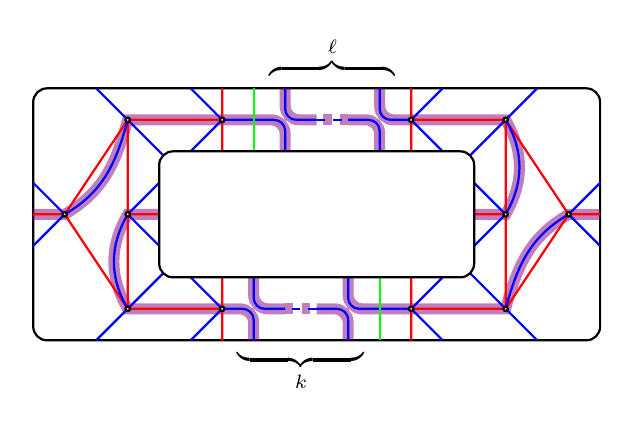
\begin{tikzpicture}[baseline=-.5ex,scale=0.4]
\draw[thick, rounded corners=5] (-9,-4) rectangle (9, 4);
\foreach \r in {0, 180} {
\begin{scope}[rotate=\r]
\begin{scope}
\draw[violet, line width=4, opacity=0.5, rounded corners=5](2,2)--(2,3)--(1,3) (0,3)--(-1,3)--(-1,4) (-1,2)--(-1,3)--(-3,3) (-3,-3)--(-2,-3)--(-2,-4);
\draw[violet, line width=4, opacity=0.5]
(-3,3)--(-6,3) to[out=-105,in=30] (-8,0) --(-9,0)
(-5,0)--(-6,0) to[out=-120,in=120] (-6,-3) -- (-3,-3);
\draw[violet, line width=4, opacity=0.5,dashed](1,3)--(0,3);
\end{scope}
\begin{scope}[yscale=-1]
\draw[thick, red]
(-3, 4) -- ++(0, -2) (-3, -4) -- ++(0, 2)
(-3, 3) -- ++(-3, 0) -- ++(0, -6) -- ++(3,0) (-6, 0) -- ++(1, 0)
(-6, 3) -- ++(-2, -3) -- ++(2, -3)
(-8, 0) -- ++(-1, 0)
;
\draw[thick, blue]
(-4, 4) -- ++(1, -1) -- ++(-1, -1) (-4, -4) -- ++(1, 1) -- ++(-1, 1)
(-7, 4) -- ++(1, -1) -- ++(1.5, -1.5) (-7, -4) -- ++(1, 1) -- ++(1.5, 1.5)
(-6, 0) -- ++(1, 1) (-6, 0) -- ++(1,-1)
(-8, 0) -- ++(-1, 1) (-8, 0) -- ++(-1, -1)
(-8, 0) to[out=-30, in=105] ++(2, -3)
(-6, 3) to[out=-120, in=120] (-6, 0)
;
\end{scope}
\draw[thick, blue, rounded corners]
(-3, 3) -- ++(2, 0) -- ++(0, -1)
(-1, 4) -- ++(0, -1) -- ++(1,0)
(2, 2) -- ++(0, 1) -- ++(-1, 0)
(-2, -4) -- ++(0, 1) -- ++(-1, 0)
;
\draw[thick, blue, dashed]
(0, 3) -- ++(1, 0)
;
\draw[thick, green] 
(-2, 4) -- ++(0,-2)
;
\draw[thick, fill=white]
(-3, 3) circle (2pt) (-3, -3) circle (2pt)
(-6, 3) circle (2pt) (-6, 0) circle (2pt) (-6, -3) circle (2pt)
(-8, 0) circle (2pt)
;
\end{scope}
}
\draw[thick, rounded corners=5, fill=white] (-5,-2) rectangle (5, 2);
\draw (0.5, 4) node[above=0ex] {$\overbrace{\hphantom{\hspace{1.6cm}}}^{\ell}$};
\draw (-0.5, -4) node[below=0ex] {$\underbrace{\hphantom{\hspace{1.6cm}}}_{k}$};
\end{tikzpicture}
}
\subfigure[$\vartheta_0({\exdynD}_{n})$]{
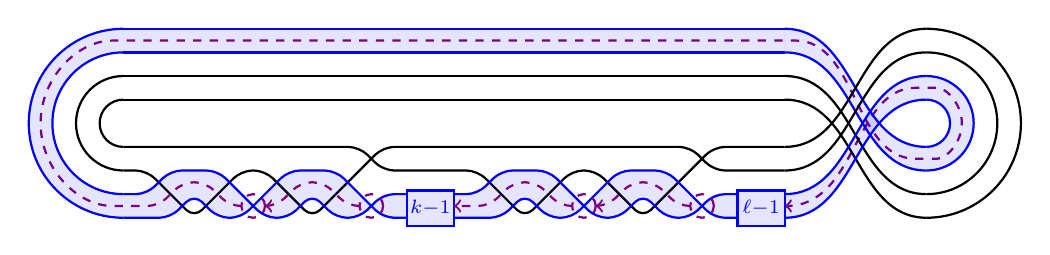
\begin{tikzpicture}[baseline=-.5ex, scale=0.6]
\begin{scope}
\draw[thick] (-7, 0.5) -- ++(7,0) (-7, 1) -- ++(7,0);
\draw[thick, blue] (-7, 1.5) -- ++(7,0) (-7, 2) -- ++(7,0);
\fill[blue, opacity=0.1] (-7, 1.5) -- ++(7,0) -- ++(0, 0.5) -- ++(-7, 0);
%
\draw[thick, rounded corners] (-7, -0.5) -- ++(0.5, 0) -- ++(4.5, 0) -- ++(0.5, -0.5) -- ++(1,0) -- ++(0.5, 0);
\draw[thick, rounded corners] (-7, -1) -- ++(0.5, 0) -- ++(1, -1) -- ++(1, 1) -- ++(0.5, 0) -- ++(1, -1) -- ++(1.5, 1.5) -- ++(1, 0) -- ++(0.5, 0);
\draw[thick, blue, rounded corners] (-7, -1.5) -- ++(0.5, 0) -- ++(0.5, 0.5) -- ++(1, 0) -- ++(1, -1) -- ++(0.5, 0) -- ++(0.5, 0.5) -- ++(0.5, -0.5) -- ++(0.5, 0) -- ++(0.5, 0.5) -- ++(0.5, 0);
\draw[thick, blue, rounded corners] (-7, -2) -- ++(0.5, 0) -- ++(0.5, 0) -- ++(0.5, 0.5) -- ++(0.5, -0.5) -- ++(0.5, 0) -- ++(1, 1) -- ++(1, 0) -- ++(1, -1) -- ++(0.5, 0);
\draw[thick, blue, fill=blue!10] (-1, -2.175) rectangle ++(1, 0.75) node[pos=.5] {$\scriptstyle k-1$};
\fill[blue, opacity=0.1] (-7, -2) [rounded corners]-- ++(0.5, 0) -- ++(0.5, 0) -- ++(0.5, 0.5) -- ++(0.5, -0.5) -- ++(0.5, 0) [sharp corners]-- ++(0.25, 0.25) 
[rounded corners]-- ++(-0.75, 0.75) -- ++(-1, 0) -- ++(-0.5, -0.5) -- ++(-0.5, 0);
\fill[blue, opacity=0.1] (-4.25, -1.75) [rounded corners]-- ++(0.75, 0.75) -- ++(1, 0) [sharp corners]-- ++(0.75, -0.75)
[rounded corners]-- ++(-0.25, -0.25) -- ++(-0.5, 0) -- ++(-0.5, 0.5) -- ++(-0.5, -0.5) -- ++(-0.5, 0) -- ++(-0.25, 0.25);
\fill[blue, opacity=0.1] (-1, -1.5) -- ++(-0.5, 0) -- ++(-0.25, -0.25) -- ++(0.25, -0.25) -- ++(0.5, 0);
%
\draw[thick, violet, dashed] 
(-4.25, -1.75) circle (0.25)
(-1.75, -1.75) circle (0.25)
;
\draw[thick, violet, dashed, ->, rounded corners]
(-2, -1.75) -- ++(-0.25, 0) -- ++(-0.5, 0.5) -- ++(-0.5, 0) -- ++(-0.5, -0.5) -- ++(-0.25, 0);
\draw[thick, violet, dashed, ->, rounded corners]
(-4.5, -1.75) -- ++(-0.25, 0) -- ++(-0.5, 0.5) -- ++(-0.5, 0) -- ++(-0.5, -0.5) -- ++(-0.75, 0) arc (-90:-270:1.75) -- ++(14, 0) to[out=0, in=180] ++(3, -2.5) arc (-90:90:0.75) to[out=180, in=0] ++(-3, -2.5);
%
\end{scope}
\begin{scope}[xshift=7cm]
\draw[thick] (-7, 0.5) -- ++(7,0) (-7, 1) -- ++(7,0);
\draw[thick, blue] (-7, 1.5) -- ++(7,0) (-7, 2) -- ++(7,0);
\fill[blue, opacity=0.1] (-7, 1.5) -- ++(7,0) -- ++(0, 0.5) -- ++(-7, 0);
%
\draw[thick, rounded corners] (-7, -0.5) -- ++(0.5, 0) -- ++(4.5, 0) -- ++(0.5, -0.5) -- ++(1,0) -- ++(0.5, 0);
\draw[thick, rounded corners] (-7, -1) -- ++(0.5, 0) -- ++(1, -1) -- ++(1, 1) -- ++(0.5, 0) -- ++(1, -1) -- ++(1.5, 1.5) -- ++(1, 0) -- ++(0.5, 0);
\draw[thick, blue, rounded corners] (-7, -1.5) -- ++(0.5, 0) -- ++(0.5, 0.5) -- ++(1, 0) -- ++(1, -1) -- ++(0.5, 0) -- ++(0.5, 0.5) -- ++(0.5, -0.5) -- ++(0.5, 0) -- ++(0.5, 0.5) -- ++(0.5, 0);
\draw[thick, blue, rounded corners] (-7, -2) -- ++(0.5, 0) -- ++(0.5, 0) -- ++(0.5, 0.5) -- ++(0.5, -0.5) -- ++(0.5, 0) -- ++(1, 1) -- ++(1, 0) -- ++(1, -1) -- ++(0.5, 0);
\draw[thick, blue, fill=blue!10] (-1, -2.175) rectangle ++(1, 0.75) node[pos=.5] {$\scriptstyle \ell-1$};
\fill[blue, opacity=0.1] (-7, -2) [rounded corners]-- ++(0.5, 0) -- ++(0.5, 0) -- ++(0.5, 0.5) -- ++(0.5, -0.5) -- ++(0.5, 0) [sharp corners]-- ++(0.25, 0.25) 
[rounded corners]-- ++(-0.75, 0.75) -- ++(-1, 0) -- ++(-0.5, -0.5) -- ++(-0.5, 0);
\fill[blue, opacity=0.1] (-4.25, -1.75) [rounded corners]-- ++(0.75, 0.75) -- ++(1, 0) [sharp corners]-- ++(0.75, -0.75)
[rounded corners]-- ++(-0.25, -0.25) -- ++(-0.5, 0) -- ++(-0.5, 0.5) -- ++(-0.5, -0.5) -- ++(-0.5, 0) -- ++(-0.25, 0.25);
\fill[blue, opacity=0.1] (-1, -1.5) -- ++(-0.5, 0) -- ++(-0.25, -0.25) -- ++(0.25, -0.25) -- ++(0.5, 0);
%
\draw[thick, violet, dashed] 
(-4.25, -1.75) circle (0.25)
(-1.75, -1.75) circle (0.25)
;
\draw[thick, violet, dashed, ->, rounded corners]
(-2, -1.75) -- ++(-0.25, 0) -- ++(-0.5, 0.5) -- ++(-0.5, 0) -- ++(-0.5, -0.5) -- ++(-0.25, 0);
\draw[thick, violet, dashed, ->, rounded corners]
(-4.5, -1.75) -- ++(-0.25, 0) -- ++(-0.5, 0.5) -- ++(-0.5, 0) -- ++(-0.5, -0.5) -- ++(-0.75, 0);
%
\end{scope}
\draw[thick] (-7, 0.5) arc (90:270:0.5) (-7, 1) arc (90:270:1);
\draw[thick, blue] (-7, 1.5) arc (90:270:1.5) (-7, 2) arc (90:270:2);
\fill[blue, opacity=0.1] (-7, 1.5) arc (90:270:1.5) -- (-7, -2) arc (-90:-270:2);
\begin{scope}
\draw[thick] (7, 1) to[out=0, in=180] ++(3, -2.5) (7, 0.5) to[out=0, in=180] ++(3, -2.5);
\draw[thick, blue] (7, 2) to[out=0, in=180] ++(3, -2.5) (7, 1.5) to[out=0, in=180] ++(3, -2.5);
\fill[blue, opacity=0.1] (7, 2) to[out=0, in=180] ++(3, -2.5) -- (10, -1) to[out=180, in=0] ++(-3, 2.5);
\end{scope}
\begin{scope}[yscale=-1]
\draw[thick] (7, 1) to[out=0, in=180] ++(3, -2.5) (7, 0.5) to[out=0, in=180] ++(3, -2.5);
\draw[thick, blue] (7, 2) to[out=0, in=180] ++(3, -2.5) (7, 1.5) to[out=0, in=180] ++(3, -2.5);
\fill[blue, opacity=0.1] (7, 2) to[out=0, in=180] ++(3, -2.5) -- (10, -1) to[out=180, in=0] ++(-3, 2.5);
\end{scope}
\draw[thick] (10, 2) arc (90:-90:2) (10, 1.5) arc (90:-90:1.5);
\draw[thick, blue] (10, 1) arc (90:-90:1) (10, 0.5) arc (90:-90:0.5);
\fill[blue, opacity=0.1] (10, 1) arc (90:-90:1) -- ++(0, 0.5) arc (-90:90:0.5);
%
\end{tikzpicture}
}
\caption{Legendrian Coxeter padding $\coxeterpadding({\exdynD}_{n})$ and the corresponding Legendrian loop $\vartheta_0({\exdynD}_{n})$}
\end{figure}

\begin{theorem}[Theorem~\ref{thm:legendrian loop}]\label{theorem:legendrian loop}
The Legendrian Coxeter mutation $\mutation_\ngraph$ on 
$(\ngraph(\exdynD),\nbasis(\exdynD))$ and twice of Legendrian mutation 
$\mutation_\ngraph^{2}$ on $(\ngraph(\exdynE),\nbasis(\exdynE))$ induce 
Legendrian loops $\vartheta(\exdynD)$ and $\vartheta(\exdynE)$ in Figures~\ref{fig:legendrian loop of E_intro} and \ref{fig:legendrian loop of D_intro}, respectively. 
In particular, the order of the Legendrian loops are infinite as elements of the fundamental group of the space of Legendrians isotopic to $\lambda(\exdynD)$ and $\lambda(\exdynE)$, respectively.
\end{theorem}

Note that the above idea of Coxeter mutation also works for $(\ngraph(a,b,c),\nbasis(a,b,c))$ with $\frac{1}{a}+\frac{1}{b}+\frac{1}{c} < 1$. Indeed the operation $\qcoxeter$ is of infinite order and so is $\ncoxeter$, hence Legendrian weaves 
\[\Legendrian(\ncoxeter^r(\ngraph(a,b,c),\nbasis(a,b,c)))\]
produce infinitely many distinct Lagrangian fillings.
The quiver $\quiver(a,b,c)$ is also bipartite and one can perform 
the Legendrian Coxeter mutation $\mutation_{\ngraph}$ on the $N$-graph $\ngraph(a,b,c)$ by stacking the gray-shaded annulus like as before. Therefore, there is no obstruction to
realize seeds obtained by mutations $\ncoxeter^r$ via the $N$-graphs.
Since the order of the Legendrian Coxeter mutation is infinite (see Lemma~\ref{lemma:order of coxeter mutation}), we obtain infinitely many $N$-graphs
and hence infinitely many exact embedded Lagrangian fillings for the Legendrian
link $\legendrian(a,b,c)$ with $\frac{1}{a}+\frac{1}{b}+\frac{1}{c} < 1$.

\begin{theorem}[Theorem~\ref{theorem:infinite fillings}]\label{thm_intro_infinite_fillings}
For each $a,b,c\ge 1$, the Legendrian knot or link $\legendrian(a,b,c)$ has 
infinitely many distinct Lagrangian fillings if
\[
\frac1a+\frac1b+\frac1c < 1.
\]
\end{theorem}

Gao--Shen--Weng \cite{GSW2020b} already proved the existence of infinitely many Lagrangian fillings for much general type of positive braid Legendrian links. Their main idea is to use the aperiodicity of \emph{Donaldson--Thomas transformation}(DT) on cluster varieties. An interesting observation is that the corresponding action of DT on the bipartite quivers in the $Y$-pattern becomes the Coxeter mutation. Accordingly, Theorem~\ref{thm_intro_infinite_fillings} can be interpreted as an $N$-graph analogue of the aperiodicity of DT.


\subsubsection{Lagrangian fillings for Legendrians of type $\dynBCFG$ or standard affine type with symmetry}
Now we move to cluster structure of type $\dynBCFG$ and standard affine types with certain symmetry.
They are obtained by the folding procedure from type $\dynADE$ or $\exdynD\exdynE$, see
Table~\ref{table:foldings}. 

In order to interpret those symmetries into Legendrians links and surfaces, we need to introduce corresponding actions on symplectic- and contact manifolds.
Consider two actions on $\sphere^3\times \R_u$, the rotation $R_{\theta_0}$ and conjugation  $\eta$ as follows:
\begin{align*}
R_{\theta_0}(z_1, z_2,u)&=(z_1\cos\theta_0 -z_2\sin\theta_0,z_1\sin\theta_0+z_2\cos\theta_0,u);\\
\eta(z_1,z_2,u)&= (\bar z_1,\bar z_2 ,u).
\end{align*}
Here $\sphere^3$ is the unit sphere in $\bbC^2$ with coordinates $z_1=r_1 e^{i\theta_1}, z_2=r_2 e^{i\theta_2}$ with $r_1^2 + r_2^2=1$.
Note that $\eta$ is an anti-symplectic involution which naturally gives $\Z/2\Z$-action on the symplectic manifold.
Under certain coordinate changes, the restrictions of $R_{\theta_0}$ and $\eta$ on $J^1\sphere^1$ become
\begin{align*}
R_{\theta_0}|_{J^1\sphere^1}(\theta,p_{\theta},z)&=(\theta+\theta_0,p_{\theta},z);\\
\eta|_{J^1\sphere^1}(\theta,p_{\theta},z)&=(\theta,-p_{\theta},-z).
\end{align*}
In turn, the rotation $R_{\theta_0}$ acts on the $N$-graph $\ngraph(\dynX)$ by rotating the disk $\disk^2$, and $\eta$ acts by flipping the $z$-coordinate.

Any $Y$-pattern of non-simply-laced finite or affine type can be obtained by folding 
a $Y$-pattern of type $\dynADE$ or $\exdynA \exdynD \exdynE$. In other words, 
those $Y$-pattern of non-simply-laced type can be seen as sub-patterns of $\dynADE$- or $\exdynA \exdynD \exdynE$-types 
consisting of $Y$-seeds with certain symmetries of finite group $G$ action. We call 
such $Y$-seeds or $N$-graphs \emph{$G$-admissible}, and the mutation in the folded 
cluster structure is a sequence of mutations respecting the $G$-orbits. 
We say that a $Y$-seed (or an $N$-graph) is \emph{globally foldable} if it is 
$G$-admissible and its arbitrary mutations along $G$-orbits are again 
$G$-admissible. 


Figure~\ref{figure:N-graph with rotational symmetry} illustrates the $N$-graphs with rotational symmetry and the corresponding $Y$-patterns of folding. Indeed, they are $\ngraph(1,n,n)$, $\ngraph(2,2,2)$, $\ngraph(3,3,3)$, $\ngraph(\exdynD_{2n})$, $\ngraph(\exdynD_4)$ which admits $\Z/2\Z$-, $\Z/3\Z$-, $\Z/3\Z$-, $\Z/2\Z$-, $\Z/2\Z$-action, respectively.

\begin{figure}[ht]
\[
\begin{tikzcd}[column sep=0.5pc, row sep=small]
\begin{tikzpicture}[baseline=-.5ex,xscale=0.5,yscale=0.5]%B_3
\draw[orange, opacity=0.2, fill] (-90:3) arc(-90:90:3) (90:3) -- (0.5,0.5) -- (-0.5,-0.5) -- (-90:3);
\draw[violet, opacity=0.1, fill] (90:3) arc(90:270:3) (270:3) -- (-0.5,-0.5) -- (0.5,0.5) -- (90:3);
\draw[thick] (0,0) circle (3);
\draw[color=cyclecolor2,line cap=round, line width=5, opacity=0.5] (-1.5,0.5) -- (-0.5, -0.5) 
(0.5, 0.5) -- (1.5, -0.5);
\draw[color=cyclecolor1,line cap=round, line width=5, opacity=0.5] (-2.5,-0.5) -- (-1.5, 0.5) (-0.5, -0.5) -- (0.5, 0.5) (1.5, -0.5) -- (2.5, 0.5);
\draw[blue, thick, fill] (0:3) -- (2.5,0.5) circle (2pt) -- (45:3) (2.5,0.5) -- (1.5,-0.5) circle (2pt) -- (-45:3) (1.5,-0.5) -- (0.5,0.5) circle (2pt) -- (90:3) (0.5,0.5) -- (-0.5, -0.5) circle (2pt) -- (-90:3) (-0.5, -0.5) -- (-1.5, 0.5) circle (2pt) -- (135:3) (-1.5, 0.5) -- (-2.5, -0.5) circle (2pt) -- (-135:3);
\draw[blue, thick] (-2.5,-0.5) -- (-180:3);
\end{tikzpicture}
&
\begin{tikzpicture}[baseline=-.5ex,xscale=0.5,yscale=0.5]%G_2
\draw[orange, opacity=0.2, fill] (0:3) arc(0:120:3) (120:3) -- (0,0) -- (0:3);
\draw[violet, opacity=0.1, fill] (0:3) -- (0,0) -- (-120:3) arc(-120:0:3) (0:3);
\draw[blue, opacity=0.1, fill] (120:3) arc(120:240:3) (240:3) -- (0,0) -- (120:3);
\draw[thick] (0,0) circle (3cm);
\draw[color=cyclecolor2, line cap=round, line width=5, opacity=0.5] (60:1) -- (45:2)  (180:1) -- (165:2) (300:1) -- (285:2);
\draw[color=cyclecolor1, line cap=round, line width=5, opacity=0.5] (0,0) -- (60:1) (0,0) -- (180:1) (0,0) -- (300:1);
\draw[red, thick] (0,0) -- (0:3) (0,0) -- (120:3) (0,0) -- (240:3);
\draw[blue, thick, fill] 
(0,0) -- (60:1) circle (2pt) -- (90:3) 
(60:1) -- (45:2) circle (2pt) -- (30:3) 
(45:2) -- (60:3);
\draw[blue, thick, fill] 
(0,0) -- (180:1) circle (2pt) -- (210:3) 
(180:1) -- (165:2) circle (2pt) -- (150:3) 
(165:2) -- (180:3);
\draw[blue, thick, fill] 
(0,0) -- (300:1) circle (2pt) -- (330:3) 
(300:1) -- (285:2) circle (2pt) -- (270:3) 
(285:2) -- (300:3);
\draw[thick, fill=white] (0,0) circle (2pt);
\end{tikzpicture}
&
\begin{tikzpicture}[baseline=-.5ex,scale=0.5]
\draw[thick] (0,0) circle (3cm);
\draw[orange, opacity=0.2, fill] (0:3) arc(0:120:3) (120:3) -- (0,0) -- (0:3);
\draw[violet, opacity=0.1, fill] (0:3) -- (0,0) -- (-120:3) arc(-120:0:3) (0:3);
\draw[blue, opacity=0.1, fill] (120:3) arc(120:240:3) (240:3) -- (0,0) -- (120:3);
\draw[cyclecolor2, line cap=round, line width=5, opacity=0.5] (60:1) -- (45:1.5) (180:1) -- (165:1.5) (300:1) -- (285:1.5);
\draw[cyclecolor1, line cap=round, line width=5, opacity=0.5] (0,0) -- (60:1) (0,0) -- (180:1) (0,0) -- (300:1) (45:1.5) -- (60:2) (165:1.5) -- (180:2) (285:1.5) -- (300:2);
\draw[red, thick] (0,0) -- (0:3) (0,0) -- (120:3) (0,0) -- (240:3);
\draw[blue, thick, fill] (0,0) -- (60:1) circle (2pt) -- (96:3) (60:1) -- (45:1.5) circle (2pt) -- (24:3) (45:1.5) -- (60:2) circle (2pt) -- (72:3) (60:2) -- (48:3);
\draw[blue, thick, fill] (0,0) -- (180:1) circle (2pt) -- (216:3) (180:1) -- (165:1.5) circle (2pt) -- (144:3) (165:1.5) -- (180:2) circle (2pt) -- (192:3) (180:2) -- (168:3);
\draw[blue, thick, fill] (0,0) -- (300:1) circle (2pt) -- (336:3) (300:1) -- (285:1.5) circle (2pt) -- (264:3) (285:1.5) -- (300:2) circle (2pt) -- (312:3) (300:2) -- (288:3);
\draw[thick, fill=white] (0,0) circle (2pt);
\end{tikzpicture}
\\
\begin{tikzpicture}[baseline=-.5ex,scale=0.7]
    
\node[Dnode] (a1) at (-2,0.5) {};
\node[Dnode] (a2) at (-1,0.5) {};
\node[Dnode] (a3) at (0,0) {};
\node[Dnode] (a4) at (-1,-0.5) {};
\node[Dnode] (a5) at (-2,-0.5) {};

\node[ynode] at (a1) {};
\node[gnode] at (a2) {};
\node[ynode] at (a3) {};
\node[gnode] at (a4) {};
\node[ynode] at (a5) {};

\draw (a1)--(a2)--(a3)--(a4)--(a5);

\node at (-3,0) {$\dynA_{2n-1}$};
\end{tikzpicture} 
&
\begin{tikzpicture}[baseline=-.5ex,scale=0.7]
\coordinate[Dnode] (d1) at (-2,0) {};
\coordinate[Dnode] (d2) at  (-1,0)  {};
\coordinate[Dnode] (d3) at (-1,0.5) {};
\coordinate[Dnode] (d4) at (-1,-0.5) {};

\foreach \y in {d1} {
	\node[ynode] at (\y) {};
}
\foreach \g in {d2,d3,d4}{
	\node[gnode] at (\g) {};
}

\draw (d1)--(d2)
(d1)--(d3)
(d1)--(d4);

\node at (-3,0) {$\dynD_{4}$};

\end{tikzpicture} 
&
\begin{tikzpicture}[baseline=-.5ex,scale=0.7]    
\node[Dnode] (a1) at (0,0) {};
\node[Dnode] (a2) at (-1,0.5) {};
\node[Dnode] (a3) at (-2,0.5) {};
\node[Dnode] (a4) at (-1,0) {};
\node[Dnode] (a5) at (-2,0) {};
\node[Dnode] (a6) at (-1,-0.5) {};
\node[Dnode] (a7) at (-2,-0.5) {};

\node[ynode] at (a1) {};
\node[gnode] at (a2) {};
\node[ynode] at (a3) {};
\node[gnode] at (a4) {};
\node[ynode] at (a5) {};
\node[gnode] at (a6) {};
\node[ynode] at (a7) {};

\draw (a1)--(a2)--(a3) (a1)--(a4)--(a5) (a1)--(a6)--(a7);

\node at (-3,0) {$\exdynE_{6}$};

\end{tikzpicture}  \\[-1em]
\rotatebox{-90}{$\rightsquigarrow$}
& \rotatebox{-90}{$\rightsquigarrow$}
&\rotatebox{-90}{$\rightsquigarrow$} \\[-2em]
\begin{tikzpicture}[baseline=-.5ex,scale=0.7]

\node at (-3,0) {$\dynB_{n}$};

\coordinate[Dnode] (1) at (-2,0) {};
\coordinate[Dnode] (2) at (-1,0) {};
\coordinate[Dnode] (3) at (0,0) {};

\node[ynode] at (1) {};
\node[ynode] at (3) {};
\node[gnode] at (2) {};

\draw (1)--(2);
\draw[double line] (2)-- ++ (3); 

\end{tikzpicture}
&
\begin{tikzpicture}[baseline=-.5ex,scale=0.7]
\node at (-3,0) {$\dynG_{2}$};
\coordinate[Dnode] (1) at (-2,0) {};
\coordinate[Dnode] (2) at (-1,0) {};

\node[ynode] at (1) {};
\node[gnode] at (2) {};

\draw[triple line] (2)-- ++ (1) ;
\draw (1)--(2);

\end{tikzpicture}
&
\begin{tikzpicture}[baseline=-.5ex,scale=0.7]
\node at (-3,0) {$\exdynG_{2}$};

\coordinate[Dnode] (3) at (-2,0) {};
\coordinate[Dnode] (2) at (-1,0) {};
\coordinate[Dnode] (1) at (0,0) {};

\node[ynode] at (1) {};
\node[gnode] at (2) {};
\node[ynode] at (3) {};

\draw (2)--(3);
\draw[triple line] (2)-- ++ (1) ;
\draw (1)--(2);

\end{tikzpicture}
\end{tikzcd}
\]

\[
\begin{tikzcd}[column sep=0.5pc, row sep=small]
\begin{tikzpicture}[baseline=-.5ex,scale=0.5]
\draw[rounded corners=5, thick] (-6.5, -2.5) rectangle (6.5, 2.5);
\draw (0.5, -2.5) %node[above] {$\cdots$} 
(-0.5, -2.5) %node[below] {$\underbrace{\hphantom{\hspace{3cm}}}_{k-2}$}
;
\draw (1.5, 2.5) %node[below] {$\cdots$} 
(0.5, 2.5) %node[above] {$\overbrace{\hphantom{\hspace{3cm}}}^{k-2}$}
;
\clip[rounded corners=5] (-6.5, -2.5) rectangle (6.5, 2.5);
\draw[orange, opacity=0.2, fill] (0,2.5)--(-7,2.5)--(-7,-2.5)--(0,-2.5);
\draw[violet, opacity=0.1, fill] (0,2.5)--(7,2.5)--(7,-2.5)--(0,-2.5);
\draw[cyclecolor1, opacity=0.5, line cap=round, line width=5] 
(-3.5, 0) -- (-2.5, 0) (-3.5, 0) -- (-4.5, 1) (-3.5, 0) -- (-4.5, -1)
(-1.5, 0) -- (-0.5, 0)
(0.5, 0) -- (1.5, 0)
(3.5, 0) -- (2.5, 0) (3.5, 0) -- (4.5, 1) (3.5, 0) -- (4.5, -1)
;
\draw[cyclecolor2, opacity=0.5, line cap=round, line width=5] 
(-4.5, 1) -- (-5.5, 1)
(-4.5, -1) -- (-4.5, -1.75)
(-1.5, 0) -- (-2.5, 0)
(-0.5, 0) -- (0.5, 0)
(1.5, 0) -- (2.5, 0)
(4.5, 1) -- (4.5, 1.75)
(4.5, -1) -- (5.5, -1)
;
\foreach \i in {0, 180} {
\begin{scope}[rotate=\i]
\draw[thick, green] (-2.5, 2.5) -- (0,0);
\draw[thick, red] 
(-3.5, -2.5) -- (-3.5, 2.5)
(-6.5, 0) -- (-3.5, 0)
;
\draw[thick, blue, fill]
(-2.5, -2.5) -- (-2.5,0) circle (2pt)
(-0.5, -2.5) -- (-0.5,0) circle (2pt)
(1.5, -2.5) -- (1.5,0) circle (2pt)
;
\draw[thick, blue, fill] 
%
(-3.5, 0) -- (3.5, 0)
(-3.5, 0) -- (-4.5, 1) circle (2pt) -- (-4.5, 2.5)
(-4.5, 1) -- (-6.5, 1)
(-5.5, 1) circle (2pt) -- (-5.5, 2.5)
%
(-3.5, 0) -- (-4.5, -1) circle (2pt) -- (-4.5, -2.5)
(-4.5, -1) -- (-6.5, -1)
(-4.5, -1.73) circle (2pt) -- (-6.5, -1.73)
;
\end{scope}
}
\draw[thick, fill=white] (-3.5, 0) circle (2pt) (3.5, 0) circle (2pt);
\end{tikzpicture}
&
\begin{tikzpicture}[baseline=-.5ex,scale=0.5]
\draw[rounded corners=5, thick] (-4, -2.5) rectangle (4, 2.5);
\clip[rounded corners=5] (-4, -2.5) rectangle (4, 2.5);
\draw[orange, opacity=0.2, fill] (0,2.5)--(-7,2.5)--(-7,-2.5)--(0,-2.5);
\draw[violet, opacity=0.1, fill] (0,2.5)--(7,2.5)--(7,-2.5)--(0,-2.5);
\draw[cyclecolor1, opacity=0.5, line cap=round, line width=5]
(-1, 0) -- (1, 0) %node[near start, above, color=black, sloped,opacity=1] {$\cycle_1$} 
(-1, 0) -- (-2, 1) (-1, 0) -- (-2, -1)
(1, 0) -- (2, 1) (1, 0) -- (2, -1)
;
\draw[cyclecolor2, opacity=0.5, line cap=round, line width=5] 
(-2, 1) -- (-3, 1) %node[midway, below, color=black,opacity=1] {$\cycle_2$}
(-2, -1) -- (-2, -1.75) %node[midway, right=-1ex, color=black,opacity=1] {$\cycle_3$}
(2, 1) -- (2, 1.75) %node[midway, left=-1ex, color=black,opacity=1] {$\cycle_4$}
(2, -1) -- (3, -1) %node[midway, above, color=black,opacity=1] {$\cycle_5$}
;
\foreach \i in {0, 180} {
\begin{scope}[rotate=\i]
\begin{scope}[xshift=2.5cm]
\draw[thick, green] (-2.5, 2.5) -- ++(0,-2.5);
\draw[thick, red] 
(-3.5, -2.5) -- (-3.5, 2.5)
(-6.5, 0) -- (-3.5, 0)
;
\draw[thick, blue, fill] 
%
(-3.5, 0) -- (-2.5, 0)
(-3.5, 0) -- (-4.5, 1) circle (2pt) -- (-4.5, 2.5)
(-4.5, 1) -- (-6.5, 1)
(-5.5, 1) circle (2pt) -- (-5.5, 2.5)
%
(-3.5, 0) -- (-4.5, -1) circle (2pt) -- (-4.5, -2.5)
(-4.5, -1) -- (-6.5, -1)
(-4.5, -1.73) circle (2pt) -- (-6.5, -1.73)
;
\end{scope}
\end{scope}
}
\draw[thick, fill=white] (-1, 0) circle (2pt) (1, 0) circle (2pt);
\end{tikzpicture}
\\
\begin{tikzpicture}[baseline=-.5ex,scale=0.7]

\coordinate[Dnode] (d1) at (0,1.5) {};
\coordinate[Dnode] (d2) at (0,0.5) {};
\coordinate[Dnode] (d3) at (1,1) {};
\coordinate[Dnode] (d4) at (2,1) {};
\coordinate[Dnode] (d5) at (3,1) {};
\coordinate[Dnode] (d6) at (0,-0.5) {};
\coordinate[Dnode] (d7) at (0,-1.5) {};
\coordinate[Dnode] (d8) at (1,-1) {};
\coordinate[Dnode] (d9) at (2,-1) {};
\coordinate[Dnode] (d10) at (3,-1) {};
\coordinate[Dnode] (d11) at (4,0) {};

\node[gnode] at (d1) {};
\node[gnode] at (d2) {};
\node[gnode] at (d4) {};
\node[gnode] at (d6) {};
\node[gnode] at (d7) {};
\node[gnode] at (d9) {};
\node[gnode] at (d11) {};

\node[ynode] at (d3) {};
\node[ynode] at (d5) {};
\node[ynode] at (d8) {};
\node[ynode] at (d10) {};

\draw  (d1)--(d3)--(d4)--(d5)--(d11)--(d10)--(d9)--(d8)--(d6)
(d2)--(d3) (d7)--(d8);

\node at (2,-2) {$\exdynD_{2n}$};
\node at (4.5,-0.1) {$\rightsquigarrow$};

\begin{scope}[xshift=5cm]
\node at (2,-2) {$\exdynB_{n}$};
\coordinate[Dnode] (1) at (0,0.5) {};
\coordinate[Dnode] (2) at (0,-0.5) {};
\coordinate[Dnode] (3) at (1,0) {};
\coordinate[Dnode] (4) at (2,0) {};
\coordinate[Dnode] (5) at (3,0) {};
\coordinate[Dnode] (6) at (4,0) {};

\node[gnode] at (1) {};
\node[gnode] at (2) {};
\node[ynode] at (3) {};
\node[gnode] at (4) {};
\node[ynode] at (5) {};
\node[gnode] at (6) {};

\draw (1)--(3)--(4)--(5) (2)--(3) ;
\draw[double line] (6)-- ++ (5) ;
\end{scope}

\end{tikzpicture}
&
\begin{tikzpicture}[baseline=-.5ex,scale=0.7]

\coordinate[Dnode] (d1) at (0,0) {};
\coordinate[Dnode] (d2) at (-1,0.5) {};
\coordinate[Dnode] (d3) at (-1,-0.5) {};
\coordinate[Dnode] (d4) at (1,0.5) {};
\coordinate[Dnode] (d5) at (1,-0.5) {};

\node[ynode] at (d1) {};
\node[gnode] at (d3) {};
\node[gnode] at (d2) {};
\node[gnode] at (d4) {};
\node[gnode] at (d5) {};

\draw (d4)--(d1)--(d2) (d3)--(d1)--(d5);

\node at (-2,0) {$\exdynD_{4}$};
\node at (0,-1) {\rotatebox[origin=c]{-90}{$\rightsquigarrow$}};

\node at (-2,-2) {$\exdynC_{2}$};
\coordinate[Dnode] (c1) at (-1,-2) {};
\coordinate[Dnode] (c2) at (-0,-2) {};
\coordinate[Dnode] (c3) at (1,-2) {};

\node[gnode] at (c1) {};
\node[ynode] at (c2) {};
\node[gnode] at (c3) {};

\draw[double line] (c3)-- ++ (c2);
\draw[double line] (c1)-- ++ (c2);

\end{tikzpicture}
\end{tikzcd}
\]
\caption{Examples of $N$-graphs with rotational symmetry}
\label{figure:N-graph with rotational symmetry}
\end{figure}

In order to present conjugation invariant $N$-graphs, we need to adopt a degenerate version of $N$-graphs which allows overlapping edges and cycles as in Figure~\ref{figure:N-graph with conjugation symmetry}.
They are equivalent to $\ngraph(\exdynD_{n+1})$, $\ngraph(\exdynD_4)$, $\ngraph(2,3,3)$, $\ngraph(3,3,3)$, and $\ngraph(2,4,4)$ up to $\partial$-Legendrian isotopy see Definition~\ref{def:boundary Legendrian isotopic}, respectively.

\begin{figure}[ht]
\[
\begin{tikzcd}[column sep=0.5pc, row sep=small]
\begin{tikzpicture}[baseline=-.5ex, scale=0.5]
\useasboundingbox (-3, -3.5) rectangle (3, 3.5);
\draw (0,0) circle (3);
\clip (0,0) circle (3);
\draw[color=cyclecolor1,line cap=round, line width=5, opacity=0.5](-135:1.5)--(45:2.5)
(-135:1.5) ++(-0.5,0) -- ++(0,-0.5);
\draw[color=cyclecolor2,line cap=round, line width=5, opacity=0.5](-135:1.5)-- ++(-0.5,0)
(-135:1.5) ++(-0.5,-0.5) -- ++(-0.5,0);
\draw[fill, red, thick]
(3,-3) -- (0,0) 
(0,0) -- (-3,3)
(0,0) -- (45:2.5) circle (2pt)
(45:2.5) -- ++(0,3) (45:2.5) -- ++(3,0)
(0,0) -- (-135:1.5) circle (2pt)
(-135:1.5) -- ++(0,-3)
(-135:1.5) -- ++(-3,0)
(-135:1.5) ++ (-.5,0) circle (2pt) -- ++(0,-2)
(-135:1.5) ++ (-.5,-.5) circle (2pt) -- ++(-2,0)
(-135:1.5) ++ (-1,-.5) circle (2pt)
(-135:1.5) ++ (-1,-.5) -- ++(0,-1);
%
\draw[Dble={green and blue},line width=2] (-2,0) -- ++(-1,-1);
\draw[Dble={green and blue},line width=2] (-2,0) -- ++(-1,1);
\draw[Dble={blue and green},line width=2] (-2,0) -- (0,0);
\draw[Dble={blue and green},line width=2] (0,0) -- (0,3);
\draw[Dble={blue and green},line width=2] (0,0) -- (0,-3);
\draw[Dble={green and blue},line width=2] (0,0) -- (2,0);
\draw[Dble={green and blue},line width=2] (2,0) -- ++(2,-2);
\draw[Dble={green and blue},line width=2] (2,0) -- ++(2,2);

\draw[color=cyclecolor3,line width=7,opacity=0.5,line cap=round](-2,0)--(2,0);
%
\end{tikzpicture}
&
\begin{tikzpicture}[baseline=-5ex,scale=0.7]

\coordinate[Dnode] (d1) at (0,0) {};
\coordinate[Dnode] (d2) at (1,0) {};
\coordinate[Dnode] (d3) at (2,0) {};
\coordinate[Dnode] (d4) at (3,0) {};
\coordinate[Dnode] (d5) at (4,0.5) {};
\coordinate[Dnode] (d6) at (4,-0.5) {};

\node[gnode] at (d1) {};
\node[ynode] at (d2) {};
\node[gnode] at (d3) {};
\node[ynode] at (d4) {};
\node[bnode] at (d5) {};
\node[bnode] at (d6) {};

\draw  (d1)--(d2)--(d3)--(d4)--(d5) (d4)--(d6);

\node at (2,0.5) {$\exdynD_{n+1}$};
\node at (2,-1) {\rotatebox[origin=c]{-90}{$\rightsquigarrow$}};

\begin{scope}[yshift=-2cm]
\node at (2,-1) {$\exdynC_{n}$};
\coordinate[Dnode] (1) at (0,0) {};
\coordinate[Dnode] (2) at (1,0) {};
\coordinate[Dnode] (3) at (2,0) {};
\coordinate[Dnode] (4) at (3,0) {};
\coordinate[Dnode] (5) at (4,0) {};

\node[gnode] at (1) {};
\node[ynode] at (2) {};
\node[gnode] at (3) {};
\node[ynode] at (4) {};
\node[bnode] at (5) {};

\draw (1)--(2)--(3)--(4) ;
\draw[double line] (5)-- ++ (4); 
\end{scope}
\end{tikzpicture}
&\hspace{6mm}&
\begin{tikzpicture}[baseline=-.5ex, scale=0.5]
\draw (0,0) circle (3);
\clip (0,0) circle (3);
\draw[color=cyclecolor1,line cap=round, line width=5, opacity=0.5](-135:2)--(45:2);
\draw[color=cyclecolor2,line cap=round, line width=5, opacity=0.5](-135:2)-- ++(-0.75,0) (45:2)--++(0.75,0);
\foreach \r in {0, 180} {
\begin{scope}[rotate=\r]
\draw[fill, red, thick]
(3,-3) -- (-3,3) 
(0,0) -- (45:2) circle (2pt)
(45:2) -- ++(0,3)
(45:2) -- ++(3,0)
(45:2) ++ (0.75,0) circle (2pt) -- ++(0,2)
;
\draw[Dble={blue and green},line width=2] (0,0) -- (0,3);
\draw[Dble={green and blue},line width=2] (0,0) -- (2,0);
\draw[Dble={green and blue},line width=2] (2,0) -- ++(-45:2);
\draw[Dble={green and blue},line width=2] (2,0) -- ++(45:2);
\end{scope}
}
\draw[color=cyclecolor3,line width=7,opacity=0.5,line cap=round](-2,0)--(2,0);
\end{tikzpicture}
&
\begin{tikzpicture}[baseline=-5ex,scale=0.7]

\coordinate[Dnode] (d1) at (0,0) {};
\coordinate[Dnode] (d2) at (-1,0.5) {};
\coordinate[Dnode] (d3) at (-1,-0.5) {};
\coordinate[Dnode] (d4) at (1,0.5) {};
\coordinate[Dnode] (d5) at (1,-0.5) {};

\node[ynode] at (d1) {};
\node[gnode] at (d3) {};
\node[gnode] at (d2) {};
\node[bnode] at (d4) {};
\node[bnode] at (d5) {};

\draw (d4)--(d1)--(d2) (d3)--(d1)--(d5);

\node at (0,0.5) {$\exdynD_{4}$};
\node at (0,-1) {\rotatebox[origin=c]{-90}{$\rightsquigarrow$}};

\node at (0,-3) {$\exdynA_{5}^{(2)}$};
\coordinate[Dnode] (c1) at (-1,-1.5) {};
\coordinate[Dnode] (c2) at (0,-2) {};
\coordinate[Dnode] (c3) at (-1,-2.5) {};
\coordinate[Dnode] (c4) at (1,-2) {};

\node[gnode] at (c1) {};
\node[ynode] at (c2) {};
\node[gnode] at (c3) {};
\node[bnode] at (c4) {};

\draw (c1)--(c2)--(c3);
\draw[double line] (c4)-- ++ (c2);
\end{tikzpicture}
\end{tikzcd}
\]
\[
\begin{tikzcd}
\begin{tikzpicture}[baseline=-.5ex, scale=0.5]
\draw (0,0) circle (3);
\clip (0,0) circle (3);
\draw[color=cyclecolor2,line cap=round, line width=5, opacity=0.5](-135:1.5)--(45:2.5);
\draw[color=cyclecolor1,line cap=round, line width=5, opacity=0.5](-135:1.5)--++(-0.5,0);
\draw[fill, red, thick]
(3,-3) -- (0,0) 
(0,0) -- (-3,3)
(0,0) -- (45:2.5) circle (2pt)
(45:2.5) -- ++(0,3) (45:2.5) -- ++(3,0)
(0,0) -- (-135:1.5) circle (2pt)
(-135:1.5) -- ++(0,-3)
(-135:1.5) -- ++(-3,0)
(-135:1.5) ++ (-0.5,0) circle (2pt) -- ++(0,-2);
%
\draw[Dble={green and blue},line width=2] (-2.5,0) -- ++(-1,-1);
\draw[Dble={green and blue},line width=2] (-2.5,0) -- ++(-1,1);
\draw[Dble={blue and green},line width=2] (-2.5,0) -- (0,0);
\draw[Dble={blue and green},line width=2] (0,0) -- (0,3);
\draw[Dble={blue and green},line width=2] (0,0) -- (0,-3);
\draw[Dble={green and blue},line width=2] (0,0) -- (1.5,0);
\draw[Dble={green and blue},line width=2] (1.5,0) -- ++(2,-2);
\draw[Dble={green and blue},line width=2] (1.5,0) -- ++(2,2);
\draw[Dble={green and blue},line width=2] (1.5,0) ++(45:0.5) -- ++(2,-2);

\draw[color=cyclecolor3,line width=7,opacity=0.5,line cap=round](-2.5,0)--(1.5,0);
\draw[color=cyclecolor4,line width=7,opacity=0.5,line cap=round](1.5,0)-- ++(45:0.5);
\end{tikzpicture} &
\begin{tikzpicture}[baseline=-.5ex, scale=0.5]
\draw (0,0) circle (3);
\clip (0,0) circle (3);
\draw[color=cyclecolor2,line cap=round, line width=5, opacity=0.5](-135:1.5)--(45:2.5) (-135:1.5)++(-0.5,0)--++(0,-0.5);
\draw[color=cyclecolor1,line cap=round, line width=5, opacity=0.5](-135:1.5)--++(-0.5,0);
\draw[fill, red, thick]
(3,-3) -- (0,0) 
(0,0) -- (-3,3)
(0,0) -- (45:2.5) circle (2pt)
(45:2.5) -- ++(0,3) (45:2.5) -- ++(3,0)
(0,0) -- (-135:1.5) circle (2pt)
(-135:1.5) -- ++(0,-3)
(-135:1.5) -- ++(-3,0)
(-135:1.5) ++ (-0.5,0) circle (2pt) -- ++(0,-2)
(-135:1.5) ++ (-0.5,0) ++(0,-0.5) circle (2pt) -- ++(-1, 0);
%
\draw[Dble={green and blue},line width=2] (-2.5,0) -- ++(-1,-1);
\draw[Dble={green and blue},line width=2] (-2.5,0) -- ++(-1,1);
\draw[Dble={blue and green},line width=2] (-2.5,0) -- (0,0);
\draw[Dble={blue and green},line width=2] (0,0) -- (0,3);
\draw[Dble={blue and green},line width=2] (0,0) -- (0,-3);
\draw[Dble={green and blue},line width=2] (0,0) -- (1.5,0);
\draw[Dble={green and blue},line width=2] (1.5,0) -- ++(2,-2);
\draw[Dble={green and blue},line width=2] (1.5,0) -- ++(2,2);
\draw[Dble={green and blue},line width=2] (1.5,0) ++(45:0.5) -- ++(2,-2);

\draw[color=cyclecolor3,line width=7,opacity=0.5,line cap=round](-2.5,0)--(1.5,0);
\draw[color=cyclecolor4,line width=7,opacity=0.5,line cap=round](1.5,0)-- ++(45:0.5);
\end{tikzpicture} &
\begin{tikzpicture}[baseline=-.5ex, scale=0.5]
\draw (0,0) circle (3);
\clip (0,0) circle (3);
\draw[color=cyclecolor2,line cap=round, line width=5, opacity=0.5](-135:1.5)--(45:2.5);
\draw[color=cyclecolor1,line cap=round, line width=5, opacity=0.5](-135:1.5)--++(-0.5,0);
\draw[fill, red, thick]
(3,-3) -- (0,0) 
(0,0) -- (-3,3)
(0,0) -- (45:2.5) circle (2pt)
(45:2.5) -- ++(0,3) (45:2.5) -- ++(3,0)
(0,0) -- (-135:1.5) circle (2pt)
(-135:1.5) -- ++(0,-3)
(-135:1.5) -- ++(-3,0)
(-135:1.5) ++ (-0.5,0) circle (2pt) -- ++(0,-2);
%
\draw[Dble={green and blue},line width=2] (-2.5,0) -- ++(-1,-1);
\draw[Dble={green and blue},line width=2] (-2.5,0) -- ++(-1,1);
\draw[Dble={blue and green},line width=2] (-2.5,0) -- (0,0);
\draw[Dble={blue and green},line width=2] (0,0) -- (0,3);
\draw[Dble={blue and green},line width=2] (0,0) -- (0,-3);
\draw[Dble={green and blue},line width=2] (0,0) -- (1.5,0);
\draw[Dble={green and blue},line width=2] (1.5,0) -- ++(2,-2);
\draw[Dble={green and blue},line width=2] (1.5,0) -- ++(2,2);
\draw[Dble={green and blue},line width=2] (1.5,0) ++(45:0.5) -- ++(2,-2);
\draw[Dble={green and blue},line width=2] (1.5,0) ++(45:0.5) ++(-45:0.5) -- ++(45:1);

\draw[color=cyclecolor3,line width=7,opacity=0.5,line cap=round](-2.5,0)--(1.5,0) (1.5,0)++(45:0.5) -- ++(-45:0.5);
\draw[color=cyclecolor4,line width=7,opacity=0.5,line cap=round](1.5,0)-- ++(45:0.5);
\end{tikzpicture}
\\
\begin{tikzpicture}[baseline=-0.5ex,scale=0.7]

\coordinate[Dnode] (d1) at (1,0) {};
\coordinate[Dnode] (d2) at (2,0) {};
\coordinate[Dnode] (d3) at (3,0.5) {};
\coordinate[Dnode] (d4) at (4,0.5) {};
\coordinate[Dnode] (d5) at (3,-0.5) {};
\coordinate[Dnode] (d6) at (4,-0.5) {};

\node[ynode] at (d1) {};
\node[gnode] at (d2) {};
\node[bnode] at (d3) {};
\node[vnode] at (d4) {};
\node[bnode] at (d5) {};
\node[vnode] at (d6) {};

\draw  (d1)--(d2)--(d3)--(d4) (d2)--(d5)--(d6);

\node at (0,0) {$\dynE_{6}$};
\end{tikzpicture} 
&
\begin{tikzpicture}[baseline=-0.5ex,scale=0.7]

\coordinate[Dnode] (d0) at (0,0) {};
\coordinate[Dnode] (d1) at (1,0) {};
\coordinate[Dnode] (d2) at (2,0) {};
\coordinate[Dnode] (d3) at (3,0.5) {};
\coordinate[Dnode] (d4) at (4,0.5) {};
\coordinate[Dnode] (d5) at (3,-0.5) {};
\coordinate[Dnode] (d6) at (4,-0.5) {};

\node[gnode] at (d0) {};
\node[ynode] at (d1) {};
\node[gnode] at (d2) {};
\node[bnode] at (d3) {};
\node[vnode] at (d4) {};
\node[bnode] at (d5) {};
\node[vnode] at (d6) {};

\draw  (d0)--(d1)--(d2)--(d3)--(d4) (d2)--(d5)--(d6);

\node at (-1,0) {$\exdynE_{6}$};
\end{tikzpicture}
&
\begin{tikzpicture}[baseline=-0.5ex,scale=0.7]

\coordinate[Dnode] (d1) at (1,0) {};
\coordinate[Dnode] (d2) at (2,0) {};
\coordinate[Dnode] (d3) at (3,0.5) {};
\coordinate[Dnode] (d4) at (4,0.5) {};
\coordinate[Dnode] (d5) at (3,-0.5) {};
\coordinate[Dnode] (d6) at (4,-0.5) {};
\coordinate[Dnode] (d7) at (5,0.5) {};
\coordinate[Dnode] (d8) at (5,-0.5) {};

\node[ynode] at (d1) {};
\node[gnode] at (d2) {};
\node[bnode] at (d3) {};
\node[vnode] at (d4) {};
\node[bnode] at (d5) {};
\node[vnode] at (d6) {};
\node[bnode] at (d7) {};
\node[bnode] at (d8) {};

\draw  (d1)--(d2)--(d3)--(d4)--(d7) (d2)--(d5)--(d6)--(d8);

\node at (0,0) {$\exdynE_{7}$};
\end{tikzpicture}\\[-1em]
\rotatebox{-90}{$\rightsquigarrow$}
& \rotatebox{-90}{$\rightsquigarrow$}
&\rotatebox{-90}{$\rightsquigarrow$} \\[-2em]
\begin{tikzpicture}[baseline=-0.5ex,scale=0.7]
\node at (0,0) {$\dynF_{4}$};
\coordinate[Dnode] (1) at (1,0) {};
\coordinate[Dnode] (2) at (2,0) {};
\coordinate[Dnode] (3) at (3,0) {};
\coordinate[Dnode] (4) at (4,0) {};

\node[ynode] at (1) {};
\node[gnode] at (2) {};
\node[bnode] at (3) {};
\node[vnode] at (4) {};

\draw (1)--(2) (3)--(4) ;
\draw[double line] (3)-- ++ (2);
\end{tikzpicture}  
&
\begin{tikzpicture}[baseline=-0.5ex,scale=0.7]
\node at (-1,0) {$\exdynE_{6}^{(2)}$};
\coordinate[Dnode] (0) at (0,0) {};
\coordinate[Dnode] (1) at (1,0) {};
\coordinate[Dnode] (2) at (2,0) {};
\coordinate[Dnode] (3) at (3,0) {};
\coordinate[Dnode] (4) at (4,0) {};

\node[gnode] at (0) {};
\node[ynode] at (1) {};
\node[gnode] at (2) {};
\node[bnode] at (3) {};
\node[vnode] at (4) {};

\draw (0)--(1)--(2) (3)--(4) ;
\draw[double line] (3)-- ++ (2) ;
\end{tikzpicture}
&
\begin{tikzpicture}[baseline=-0.5ex,scale=0.7]
\node at (0,0) {$\exdynF_{4}$};
\coordinate[Dnode] (1) at (1,0) {};
\coordinate[Dnode] (2) at (2,0) {};
\coordinate[Dnode] (3) at (3,0) {};
\coordinate[Dnode] (4) at (4,0) {};
\coordinate[Dnode] (5) at (5,0) {};

\node[ynode] at (1) {};
\node[gnode] at (2) {};
\node[bnode] at (3) {};
\node[vnode] at (4) {};
\node[bnode] at (5) {};

\draw (1)--(2) (3)--(4)--(5) ;
\draw[double line] (3)-- ++ (2) ;
\end{tikzpicture}
\end{tikzcd}
\]
\caption{Examples of $N$-graphs with conjugation symmetry}
\label{figure:N-graph with conjugation symmetry}
\end{figure}

\begin{theorem}[Theorem~\ref{thm:folding of N-graphs}]\label{Thm:folding of N-graphs}
The following holds:
\begin{enumerate}
\item The Legendrian $\lambda(\dynA_{2n-1})$ has $\binom{2n}{n}$ Lagrangian fillings which are invariant under the $\pi$-rotation and  admit the $Y$-pattern of type $\dynB_n$.
\item The Legendrian $\lambda(\dynD_{4})$ has $8$ Lagrangian fillings which are invariant under the $2\pi/3$-rotation and admit the $Y$-pattern of type $\dynG_2$.
\item The Legendrian $\lambda(\exdynE_{6})$ has Lagrangian fillings which are invariant under the $2\pi/3$-rotation and admit the $Y$-pattern of type $\exdynG_2$.
\item The Legendrian $\lambda(\exdynD_{2n})$ with $n\ge 3$ has Lagrangian fillings which are invariant under the $\pi$-rotation and admit the $Y$-pattern of type $\exdynB_n$.
\item The Legendrian $\lambda(\exdynD_4)$ has Lagrangian fillings which are invariant under the $\pi$-rotation and admit the $Y$-pattern of type $\exdynC_2$.
%
\item The Legendrian $\tilde\lambda(\dynE_{6})$ has $105$ Lagrangian fillings which are invariant under the antisymplectic involution and admit the $Y$-pattern of type $\dynF_4$.
\item The Legendrian $\tilde\lambda(\dynD_{n+1})$ has $\binom{2n}{n}$ Lagrangian fillings which are invariant under the antisymplectic involution and admit the $Y$-pattern of type $\dynC_n$.
\item The Legendrian $\tilde\lambda(\exdynE_{6})$ has Lagrangian fillings which are invariant under the antisymplectic involution and admit the $Y$-pattern of type $\dynE_6^{(2)}$.
\item The Legendrian $\tilde\lambda(\exdynE_{7})$ has Lagrangian fillings which are invariant under the antisymplectic involution and admit the $Y$-pattern of type $\exdynF_4$.
\item The Legendrian $\tilde\lambda(\exdynD_4)$ has Lagrangian fillings which are invariant under the antisymplectic involution and admit the $Y$-pattern of type $\dynA_5^{(2)}$.
\end{enumerate}
\end{theorem}

The study of Lagrangian fillings with symmetry, again to the best of authors' knowledge, is started from \cite{Cas2020}. We clarify the actions on the symplectic and contact manifold, together with the induced actions on Lagrangian fillings and Legendrian links. The items (1),(2),(6),(7) in Theorem~\ref{Thm:folding of N-graphs} answer that the conjecture \cite[Conjecture 5.4]{Cas2020} is true, and furthermore we extend our results to certain non-simply-laced affine types.


\subsection{Organization of the paper}
The rest of the paper is divided into six sections including appendices. 
We review, in Section~\ref{sec:cluster algebras}, some basics on finite and affine cluster algebra. Especially we focus on structural results about the combinatorics of exchange graphs using Coxeter mutations.

In Section~\ref{sec:N-graph}, we recall how $N$-graphs and their moves encode Legendrian surfaces and the Legendrian isotopies. We also introduce degenerate $N$-graphs which will be used to construct Lagrangian fillings having conjugation symmetry. 
After that we review the assignment of $Y$-seeds in the cluster structure from $N$-graphs together with certain flag moduli. We also discuss the Legendrian mutation on (degenerate) $N$-graphs.

In Section~\ref{sec:N-graph of finite or affine type}, we investigate Legendrian links and $N$-graphs of type $\dynADE$ or $\exdynD \exdynE$. 
We discuss $N$-graph realization of the Coxeter mutation and prove Theorem~\ref{theorem:legendrian loop} on the relationship between Coxeter mutations and Legendrian loops.
By combining the structural results in the seed pattern of cluster algebra and $N$-graph realization of the Coxeter mutation, we construct as many Lagrangian fillings as seeds for Legendrian links of type $\dynADE$ or $\exdynD \exdynE$, and hence prove Theorem~\ref{thm_intro_1}.

In Section~\ref{section:folding}, we discuss rotation and conjugation actions on $N$-graphs and invariant $N$-graphs. We also prove Theorem~\ref{Thm:folding of N-graphs}.

In Appendix~\ref{section:invariance and admissibility}, 
we argue that $G$-invariance of type $\dynADE$ implies $G$-admissibility. 
Finally, in Appendix~\ref{sec:supplementary pictorial proofs}, we collect several equivalences between different presentation of $N$-graphs.

If some readers are familiar with the notion of cluster algebra and $N$-graph, then one may skip Section~\ref{sec:cluster algebras} and Section~\ref{sec:N-graph}, respectively, and start from Section~\ref{sec:N-graph of finite or affine type}.


\subsection*{Acknowledgement}
B. An and Y. Bae were supported by the National Research Foundation of Korea (NRF) grant funded by the Korea government (MSIT) (No. 2020R1A2C1A0100320).
E. Lee was supported by the Institute for Basic Science (IBS-R003-D1).

